\subsection{03.09.2011 Samstag}
\begin{wrapfigure}{R}{0.45\textwidth} 
  \begin{centering}
    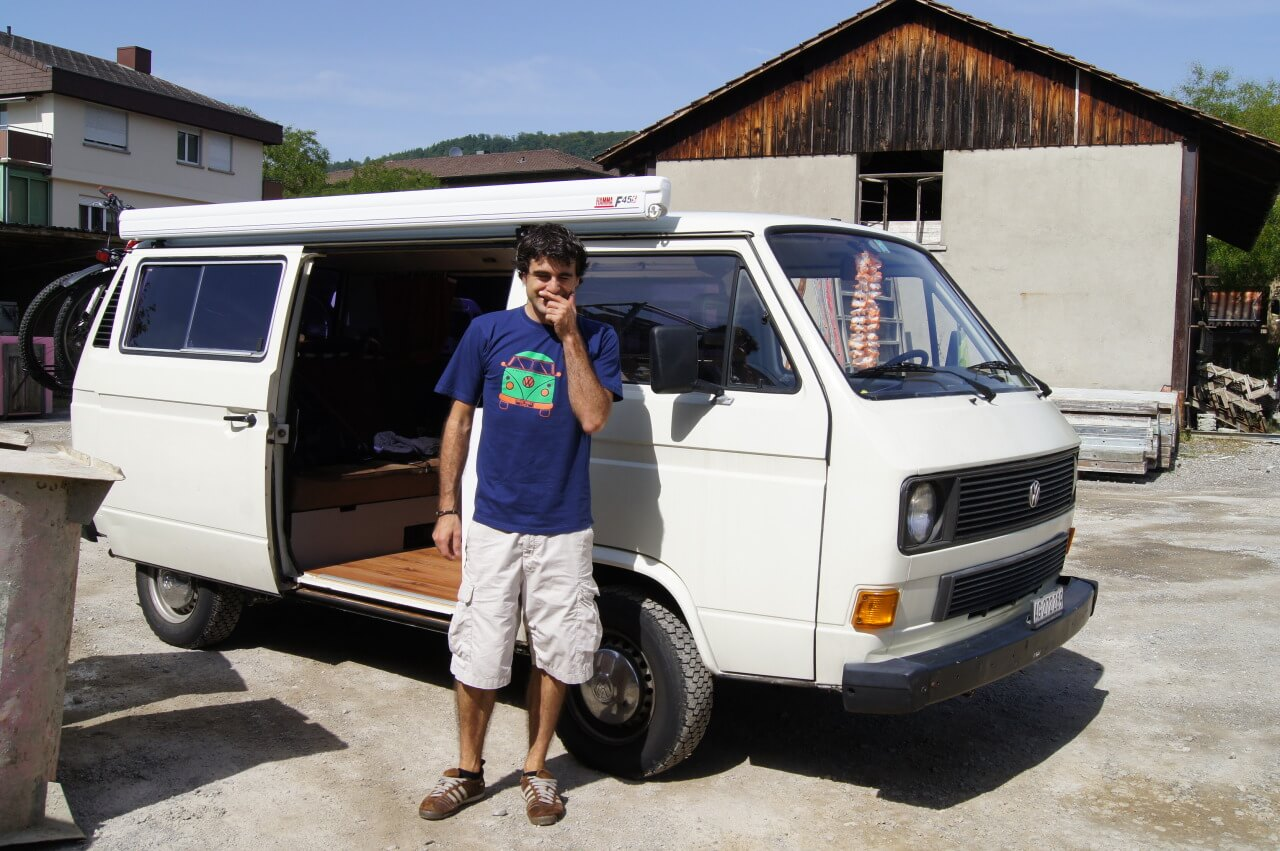
\includegraphics[width=0.4\textwidth, height=5cm, keepaspectratio]{../Bilder/Korsika/1.jpg}
    \caption{Uf gohts}
  \end{centering}
\end{wrapfigure} 
Morgenstund hat Gold im Mund... oder  au ned ;-) Am halbi 10ni simer öpe ufgstande und hend zersch mal gmüetlich zmörgelet.
Da de Jack und de Philipp sehr gmüetlichi send, hends mer ja au chli chillig chöne neh;-) Scho am halbi 3 semer de startklar gsi und hend euse Jack vollglade...juhuuu, eusi erscht gross Reis met em Büsli cha afo! En Weggis hemer scho de erscht Stopp igleit und send chli an See ghöklet und hend öpis gesse und trunke.
Esch superschön gsi und sWetter esch traumhaft gsi.
Nach Weggis ha ich de mini Fahrkönst welle zeige und be uf de Achsestross umedüsed...alli hend seeehr Freud a mer gha, well ich natürli en Speedy Consalez gsi ben:P
Vorem Gotthard, wos echli stockend witergange esch, send mini Nerve scho am Endi gsi und de Herr Bopp het müesse witerfahre.
Mer send dor de Gotthard düsed Richtig Italia...und sWetter esch emmer besser worde...chum send mer es Tessin cho hets afo seiche; dasch eus zemli bekannt vorcho.
E de erschte Raststätt em Tessin hets zNacht ge und zwar zwoi sehr chlini Portione Lasagne und Tortellini.
Meteme volle Mage und eme halbe Swimmingpool e eusem Büsli hemer die italienisch Grenze souverän öberquert.
Zemli lang semer uf donkle, met Grillesound umgebni Strasse umekurvt bes mer denn dAutobahn gfonde hend.
Um di 10ni hemer de gfonde mer send för höt gnueg uemdüst und send e Stond vor Genua ufe Raststätt go öbernachte.
Ruckzuckzackzack hemer euses Bettli parat gha und hend eus ed Decki chöne imulme.
dNacht esch echli unruhig gsi, neb de velle Autos wo cho und gange send, hend es paar obercooli Gangster gmeint sie müsset ihri Mega-Boom-Boom-Musig en aller Lutstärki eus abspele. 

\subsection{04.09.2011 Sonntag}
\begin{wrapfigure}{L}{0.45\textwidth} 
  \begin{centering}
    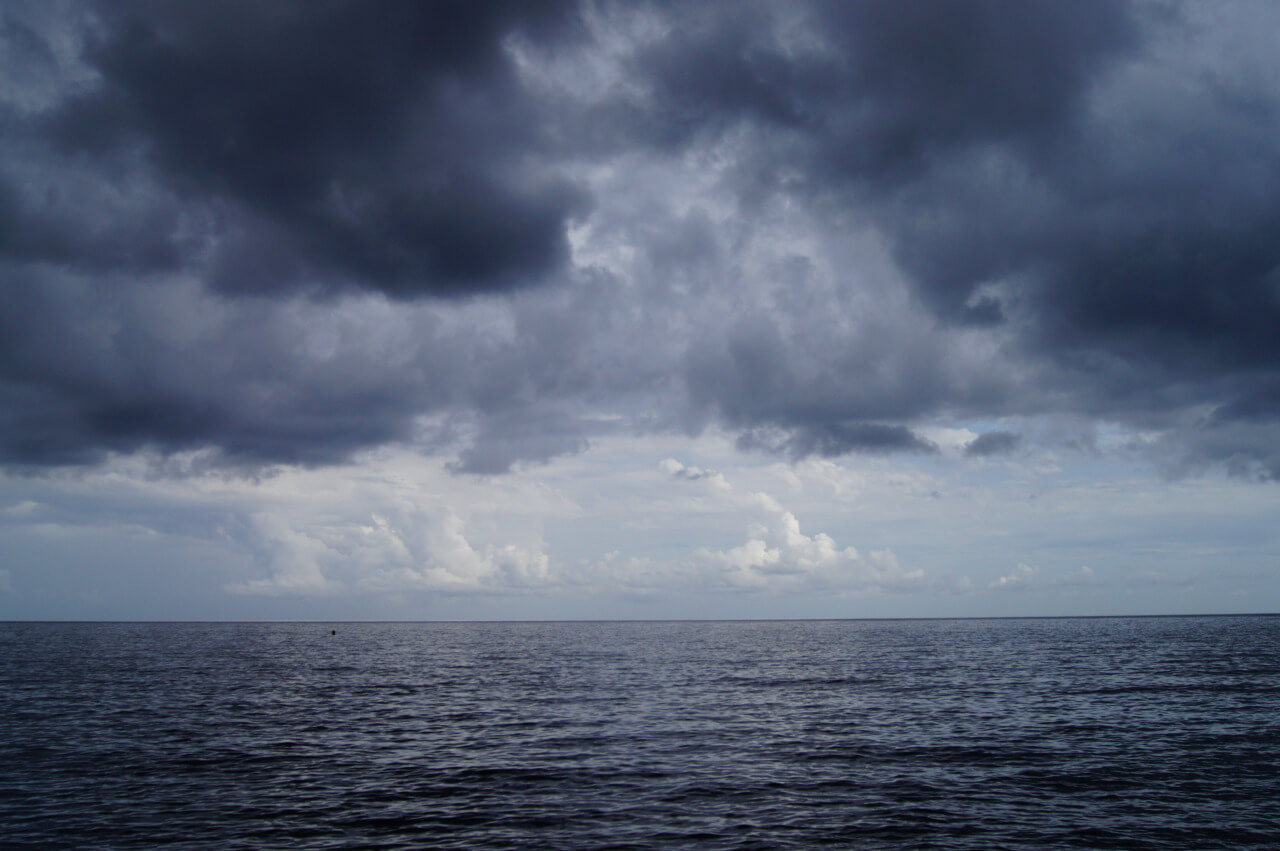
\includegraphics[width=0.4\textwidth, height=5cm, keepaspectratio]{../Bilder/Korsika/3.jpg}
    \caption{Nasser Empfang}
  \end{centering}
\end{wrapfigure} 
Höt esch fertig gsi met der Gemütlichkeit...
versuchs mal mit Gemütlichkeit, mit Ruhe und Gemütlichkeit ;) scho am halb 6i semer ufgstande, hend gschnell zmörgelet und send de schnell uf Genua düset.
De Steff und de Jack het freud gha de kurveriche Autobahn.
Ich ha schochli Angst gha, dass mer eusi Fähri verpasset, well ufem Ticket staht, dass mer 90min vor Abfahrt scho muess ischiffe...
aber mer send pönktlich, vellecht fasch zu pönkltich för Italiener, be euse Moby Wonder acho und setzted jetzt grad ufem Deck und gnüssed die schön Ussecht und dRegetröpfli und de Wind ;) Aber siehe da dSonne esch de doch na vörecho und mer hend nachli chöne sönnele e eusne Liegestüehl.
Plötzlich hemer e chlini Insle und Elba erspäht und schlussendlich au Korsika...Korsika we are coming:) 
Met euse chline Fähri semer en Hafe vo Bastia manövriert.
Trotz emene müehsame Alarmsignal esch alles guet gange und euse Jack esch gsond und ufem korsische Festland acho.
Mer send geg de Strom en Norde ufegfahre Richtig Cap Corse.
En Erbalunga hemer euse erscht Stopp gmacht und send dor die superschöne Altstadt bis zum Hafe gschlenderet.
Vo allem Mögliche hemer müesse es Föteli mache ;)... alti gelb-orangi-toskanisch-aghuchti Hüsli, romantischi engli Gässli und vell herzigi Kaffis und Restaurants.
Aber leider hend eus dRegetröpfli oder besser gseit riesigi Regetropfe bis nach Korsika verfolgt...wo mer am Hafe unde gsi send hets afo Tröpfelet.
Gli hets afo Seiche und er send zum Jack zruggsecklet.
Denn eschs ersch recht losgange, de Petrus hets guet met eus gmeint, es esch emmer meh cho regne bis euse Jack eme Boot gliche het....
be mer hets sogar inegsprudlet!! Aber dor die superbreite und guet preparierte Strosse esch da ja ke Problem gsi.
Eigentli hemer welle en Macciagio öbernachte, aber da eusi Sicht ja biizli igschränkt gsi esch, hemer de Campingplatz verpasst.
Mer send tapfer witergfahre und send de ad Westküste cho...
ah ja da eschs Wetter ja vell besser gsi;) Jetzt semer au na fasch devogfloge! Aber damol hemer dAbzwigig för de Campingplatz en Centuri-Port ned verpasst und send das schmale Wegli bes zum Meer abekurvt.
De Campingplatz esch u herzig gsi, klein aber oho.
Mer hend eusi super Usrüstig met Store natürli ufbaut, send go dusche und hend eus uf de Weg nacheme Restaurant gmacht...
leider ned erfolgrich.
Devör hemer en wonderschöne Sonneuntergang am Hafe unde chöne gnüsse.
Uf de Suechi nach Esse semer weder zo eusem Camping ufegloffe und damal hemer Glöck gha....
hmmm ufere chline Terrasse hemer fein gschlemmeret...
Entercote, Calamari, Frites und e Fläsche Wii ;) Gschlafe hemer tüüüf und fescht, gwössi Persone send grad en Ohmacht gfalle;)

\begin{figure}[hb]
    \centering
    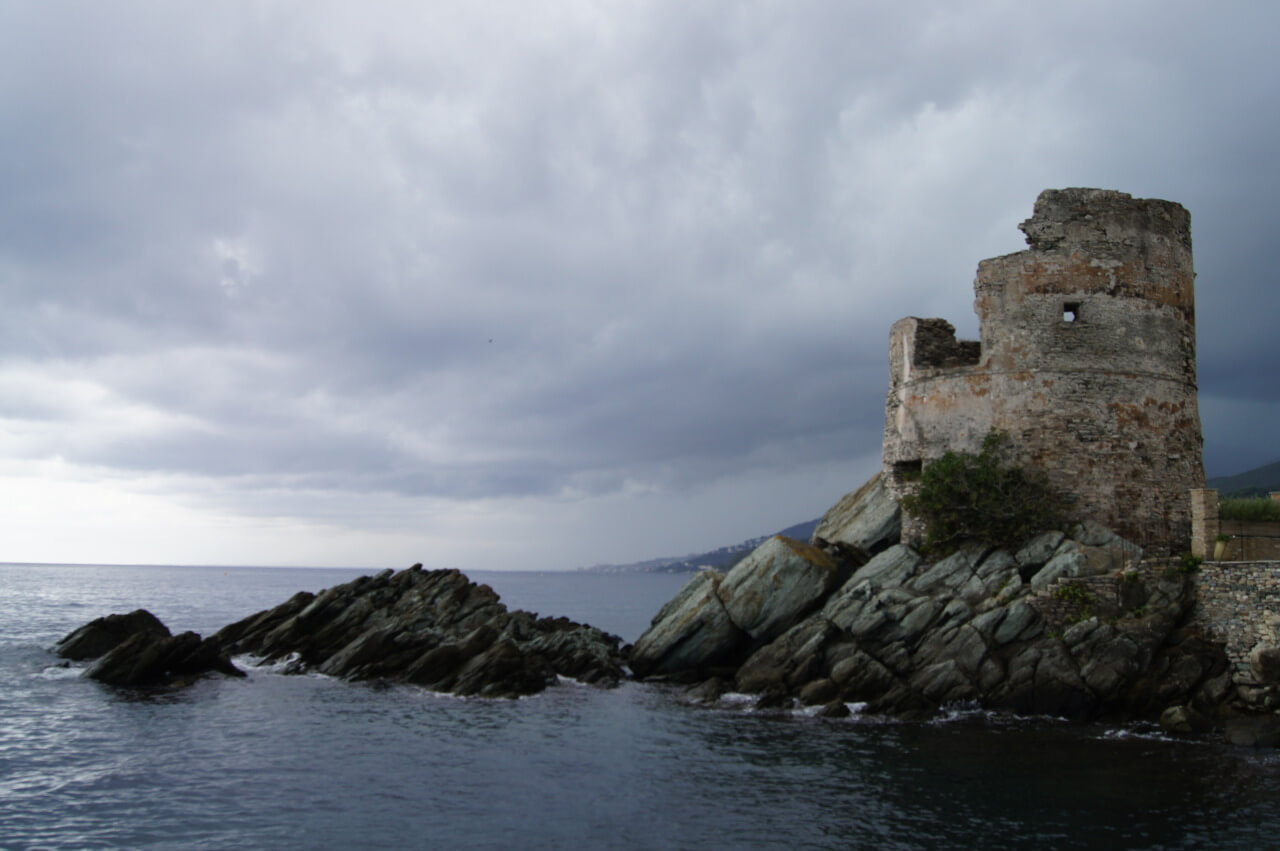
\includegraphics[width=\textwidth]{../Bilder/Korsika/4.jpg}
    \caption{Wetter het no Rum zur Verbesserig}
    \label{img:Korsika1}
\end{figure}

\pagebreak

\subsection{05.09.2011 Montag}

\begin{wrapfigure}{L}{0.45\textwidth} 
  \begin{centering}
    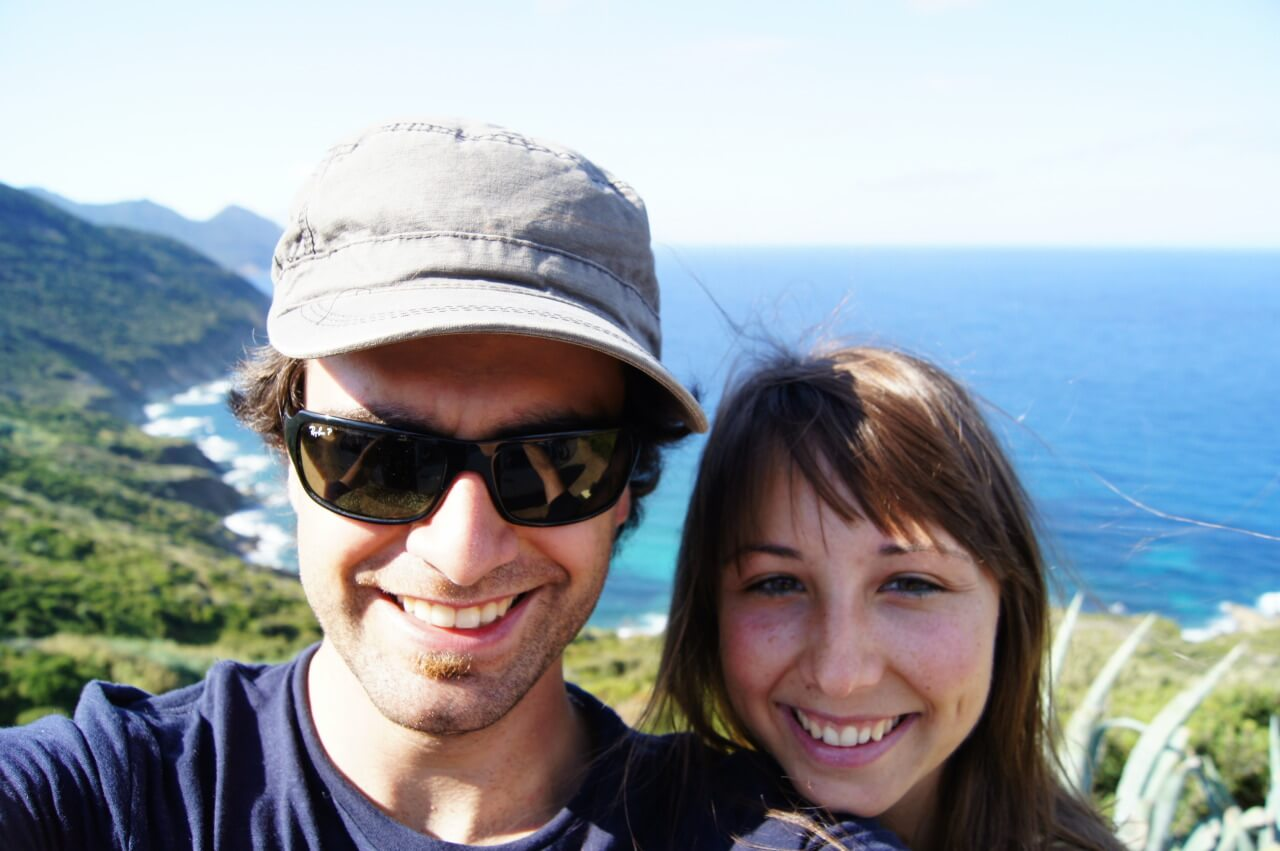
\includegraphics[width=0.4\textwidth, height=5cm, keepaspectratio]{../Bilder/Korsika/6.jpg}
    \caption{Zwei Entdecker uf Korsika}
  \end{centering}
\end{wrapfigure} 

\begin{figure}[b]
   \centering
      %\subfloat[CAPTION]{BILDERCODE}\qquad
   \subfloat{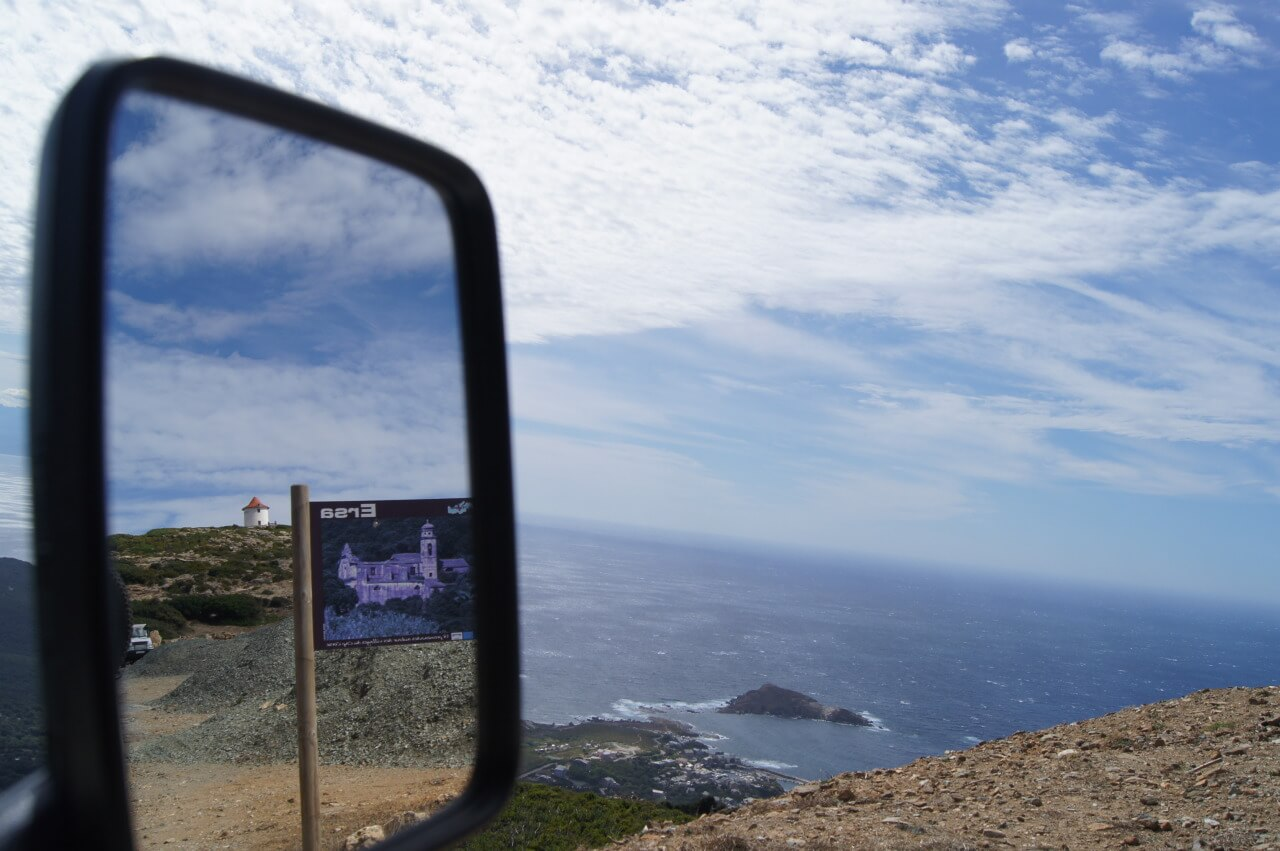
\includegraphics [width=0.3\textwidth]{../Bilder/Korsika/7.jpg}}\quad
   \subfloat{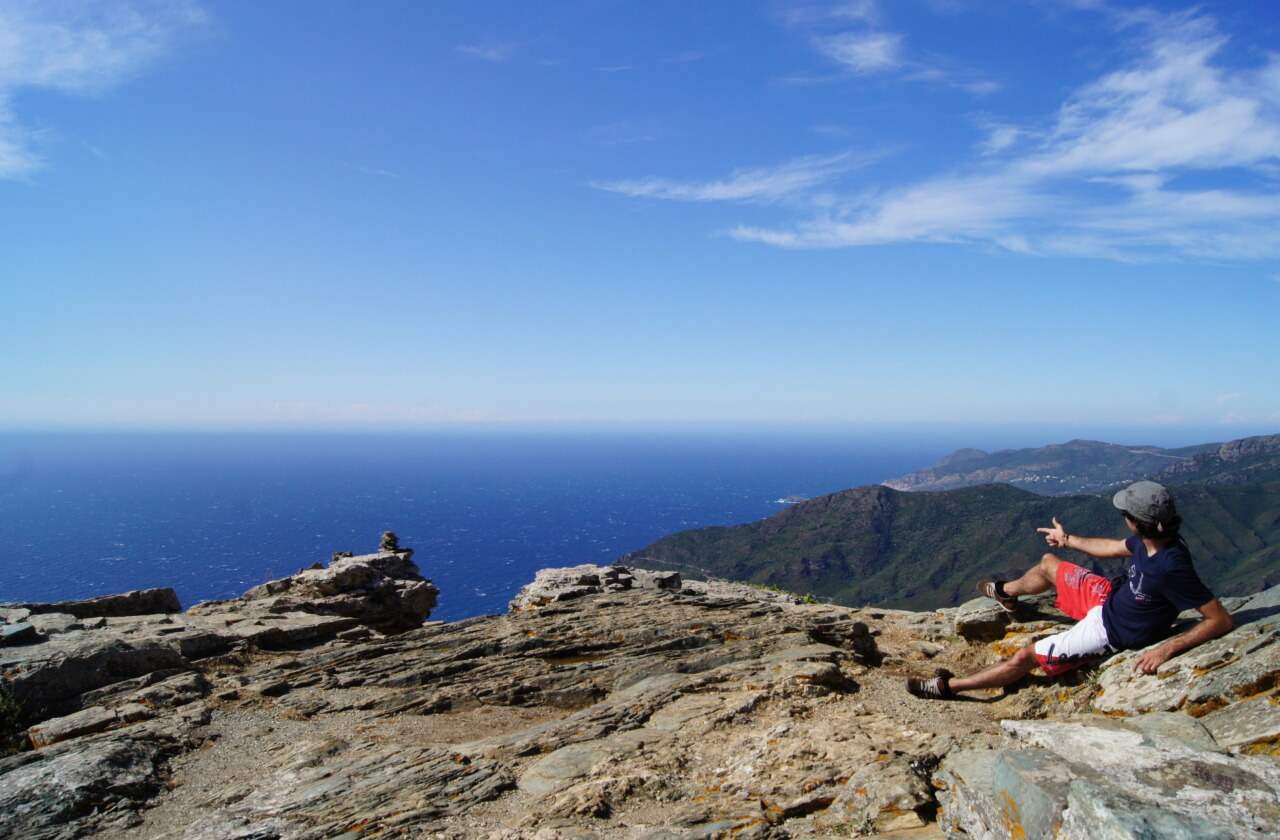
\includegraphics [width=0.3\textwidth]{../Bilder/Korsika/11.jpg}}\quad
   \subfloat{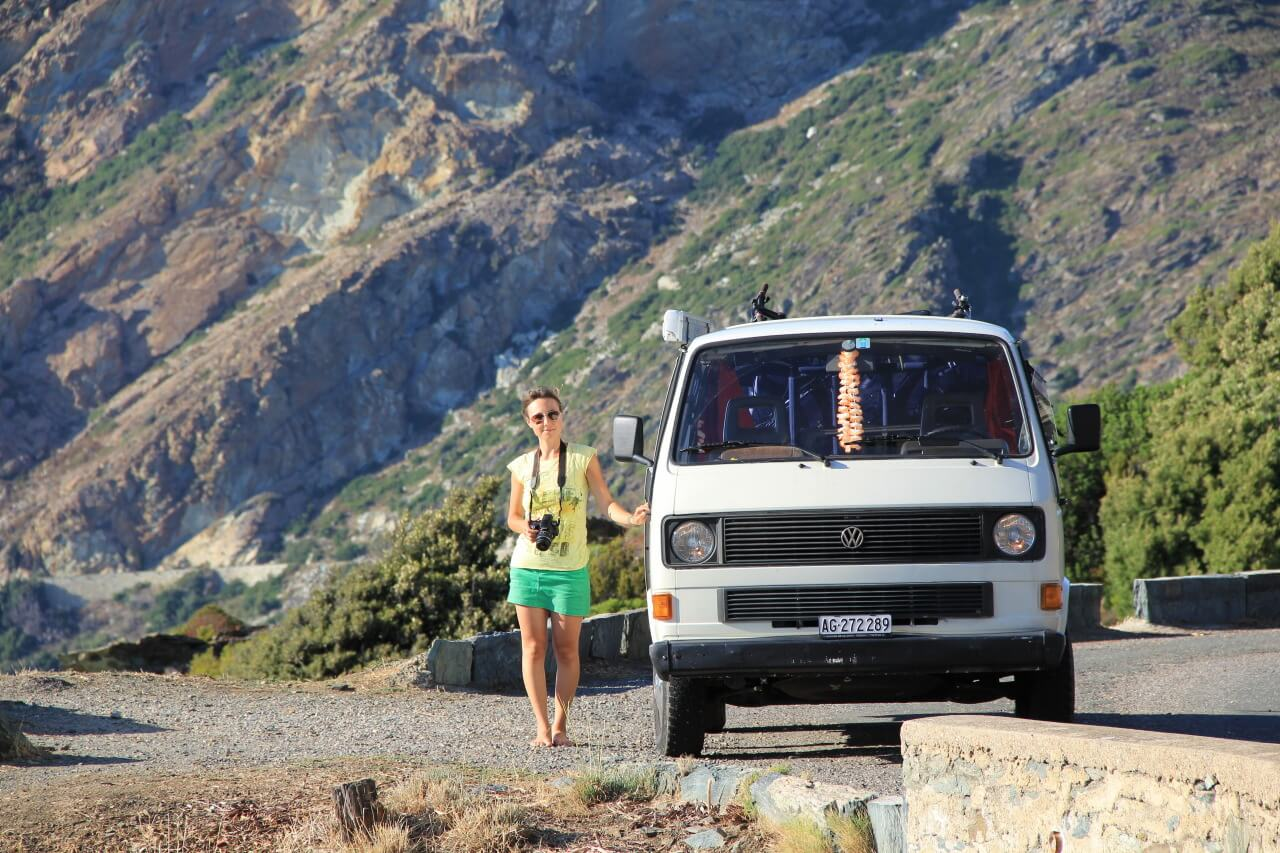
\includegraphics [width=0.3\textwidth]{../Bilder/Korsika/12.jpg}}\quad
   \caption[Korsika wie im Birlderbuech]{Korsika wie im Bilderbuech}
\end{figure}
Sonnen-Sonnen-Sonnenschein :-) In aller Frische und met eme chline Durscht semer um di 9ni ufgstande.
Zum zMorge hets suuuperfeini Croissant und en starke Kaffi ge.
Nach dem Kaffi hemer euses Büsli so schnell wie no nie ufgrumet gha und mer send back to the road an nördlichst Ponkt vo Korsika uf Barcaggio gfahre.
Vo Ersa het wedermal es sehr abentürlichs Strösslii ad Küste gführt.
De Jack und de Superdriver hend das aber super gmeisteret und mer send belohnt worde met ere wonderschöne Bucht met de Insle Giraglia im Hintergund und emene ned allzu schöne Strand.
Jetzt hets gheisse: sönnele, usruhe und vor allem Bädele...hihi...ich kenn da öper wo sich nachem Bädele gsehnt het und de nor bes zode Chnü es Wasser esch und de scho gnueg vom Bade gha het;) sWasser esch glasklar gsi und mer hätt wit use chöne laufe.
Mer send de aber em Strand noche Richtig Genueseturm gloffe und hend na es chlises Restaurant gfonde, wo mer öpis trunke hend.
De semer au scho gli weder gange, well mer na es rechts Programm vor eus gha hend...nor hemer ned gwösst das das au e Wanderig beinhaltet;) Mer send alles de Köste entlang Richtig Pino gfahre und hend ufem Weg vell chlini herzigi Bergdörfli atroffe.
En Pino send mer abboge för uf de Seneca-Ussechts-Turm.
Anstatt es winzigs Strössli wo mer erwartet hend, hets e schöni terreti Stross gha.
Scho vo witem hemer de Turm in weiter Höhe obe gseh, aber dStross het de leider gar nöm so höch ufegführt und mer hend müesse zFuess witerga, obwohl de Turm emmer recht wit obe gsi esch.
Euse Wanderer het gmeint es göch 2 Stond und dOptimistin het met 30min grechnet..schlussendlich sends öpe 40 Minute gsi, wo mer steil de Berg hend müesse ufeklettere.
Teilwis hemer wörkli müesse eusi Chletterkönst uspacke und hend chli zwiflet, öb das wörkli de rechtig Weg esch.
Dobe acho semer de met ere wooonderschöne Ussecht belohnt worde.
dOst- und Westküste vom Cap Corse und die schön hügelig Landschaft em Landesinnere hend mer chöne bestune.
Natürli ha ich grad es paar Panoramas müesse schüsse.
Nacheme usgibige Fotoshooting hemer de Abstig en Agriff gno und send de rechtig St.Florent düset.
Nach Nonza hemer de euse Campingplatz A Stella gfonde.
Dummerwis semer ned grad direkt ad Rezeption gfahre, was dFrau Rezeptionistin alias Hilfsherif gar ned lostig gfonde het.
Sie het sich fasch nöm chöne erhole, het eus de aber doch na dErlaunis ge zum öbernachte.
Mer hend eus de au en super Platz direkt vorem Strand ade pole position gsicheret.
Es esch zwar chli schief gsi, aber mer hend e traumhafti Ussecht ufs wilde Meer gha.
De Sonneuntergang hemer met eme Campari und Chips uf eusne Ligistühe gnosse.
Zum Znacht hets Tomatesalat met Brot und Korsische Worscht ge.
Nachem Esse hend mer de Sternehimmel bestunt und jeglichi Sternschnuppe, Satellite und sogar Ufos erspäht;-) Nachem Sternegucke und Philosophiere send mer de meteme schöne (bizli lute) Wellerusche zfride ipfused.

\subsection{06.09.2011 Dienstag}
\begin{wrapfigure}{L}{0.45\textwidth} 
  \begin{centering}
    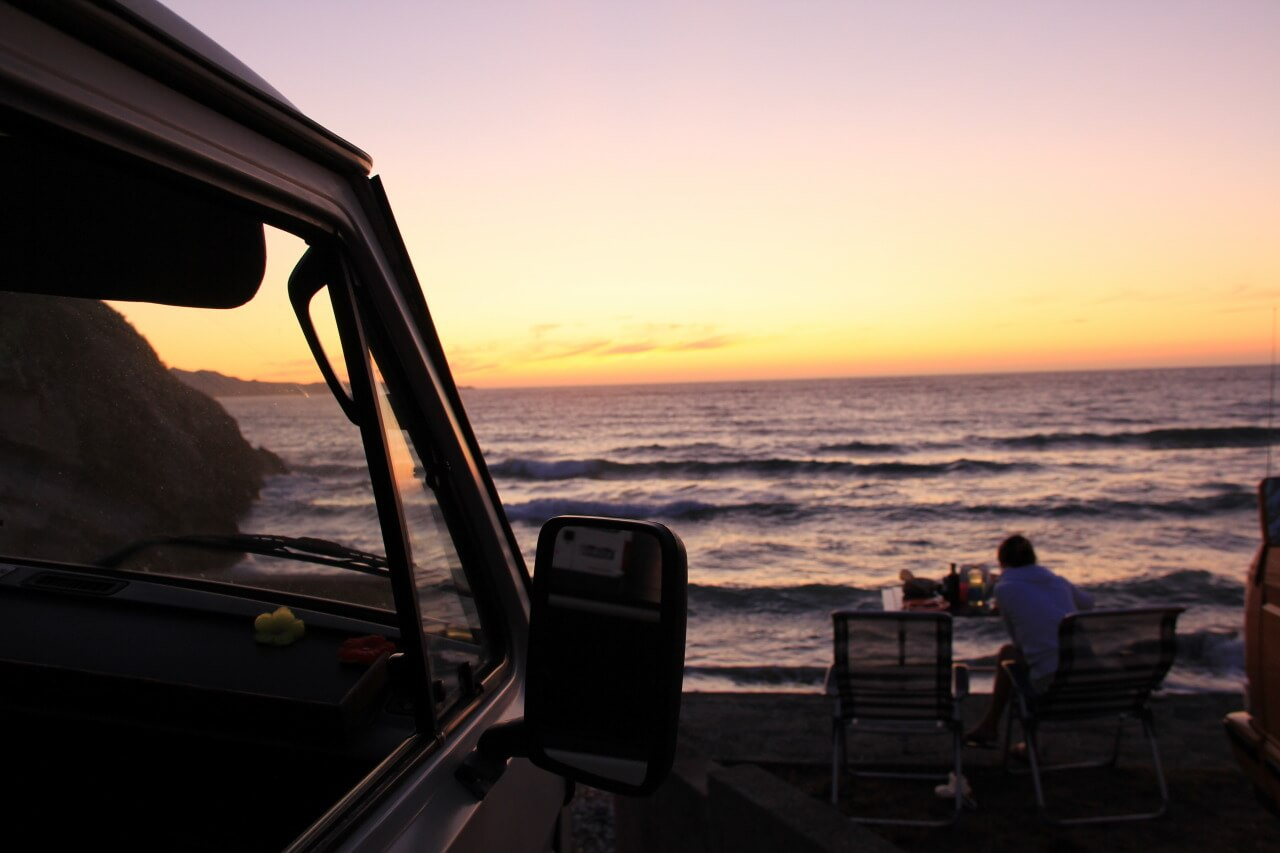
\includegraphics[width=0.4\textwidth, height=5cm, keepaspectratio]{../Bilder/Korsika/18.jpg}
    \caption{Zwei Entdecker uf Korsika}
  \end{centering}
\end{wrapfigure} 
Au ufgwacht semer metemene rusche... Wellerusche :) zMörgelet hemer met ere geniale Ussecht uf die schön Bucht und send de au scho gli wederemal loszottlet.
A St.Florent semer verbigurket, well mer grad chli gschockt gsi send vo de velle Lüt wos döt gha het;) Witer Rihtig Ille Rousse hemer es paar wonderschöni Stränd gsichtet und send de be de vo Lozuri go bädele.
Es het recht grossi Welle gha und de Steff het mer fasch nöm chöne usem Wasser bringe....ich be rechtig erstunt gsi und has chum chöne glaube.
Nach erschte skeptische Anöcherige het er sich vode Welle nöme chöne trenne und esch am Strand em Welletakt ufe und abegrugelet....oh Wunder das er nacher e halbi Tonne Sand e sinere Hose gha het;-) Nachem Bädele und Sönnele semer de witer und hend en Ille Rousse en Stop gmacht.
WOW...die rote Granitfelse em türkisblaue Wasser hend eifach traumhaft usgseh! Mer hend en Spaziergang (met echli chlettere) zum Genuese- und Lüchtturm gmacht, wo mer eifach en grandiosi Ussecht ufs Städtli und die karibikähnliche Buch gha hend.
Denn hemer en feini Crepes verschlunge und send nach Calvi gfahre.
Em grosse und schöne Campingplatz La Pinede hemer eus niederglo, hend eus früsch gmacht und send met em Velo ed Downtown Calvi gfahre.
Em Strand und de Isebahngleis nache semer düset und hend en superschöni Ussecht uf Zitadelle vo Calvi gha.
Calvi esch en mega herzigi und touristischi Stadt met herzige Gässli, Lädeli, vellne Gelati-Ständ und schöne Restaurant am Hafe entlang.
Mer send enes Restaurant, wo em Reiseführer empfole worde esch und es esch eifach genial gsi...hmm de Steff het Teigware met Meeresfröcht gha und ich Lachs met Ris und Gmües. himmlisch:) Glöcklich und met vollem Buch semer zom Camping zrugfahre und send go pfuuuse. 

\subsection{07.09.2011 Mittwoch}

sErscht mal hemer 2 Nächt uf eim Camping öbernachtet und so hemer en super gmüetliche Tag gmacht en Calvi.
Schön usgschlafe hemer, fein zmörgelet und de semer met de Velos es Altstädtli vo Calvi düset.
Zersch semer go Zidatelle aluege, was zemli imposant gsi esch.
Neb de hoche Mure hets ganz vell schöni Sujets vo alte Hüser, Fenster und Töre gha zum Fotografiere, mer zwoi Hobbyfotografe hend nöm welle ufhöre met Fötele;) De Innehof vode Zidatelle esch na zemli gross gsi und es het so usgseh, wie na Lüt e dene alte Hüser läbet.
Die Zitadelle und die velle Genuesetürm send na Relikt vode genuesische Herrschaft, wo fasch es Jahrhundert öber Korsika regiert hend.
Nach dem spannende Rundgang semer zrug zo eusem Camping hend eusi Bad- und Schnorchelsache ipackt und send an Strand.
Döt hemer gsönnelet, bädelet und sogar gschnorchlet! Em Meer hesch mega wit use chöne laufe..
de Steff esch fasch de ganz Weg met de Flosse usegwatschlet;) Bem Schnorchle hemer paar schöni selbrigi Fisch gseh und de Steff het sogar en Tintefisch gseh, angeblich;) Ich ha nüt gseh, well de Steff so umegfuchtlet het, dass er mit sine Flosse en ganze Sandstorm veranstaltet het;) Nach dem astrengende Schnorchle semer zo eusem Jack zrug und hend fein zNacht kochet: Spaghetti met Carbonara-Sauce.
Korsische Wy hemer na kauft, aber leider esch de zemli sur gsi.
Es esch super gmüetlich gsi und mer hend gnueg Zyt gha zum die andere Camper (vor allem Däne) met erne Töff zbeobachte.

\begin{figure}[H]
    \centering
    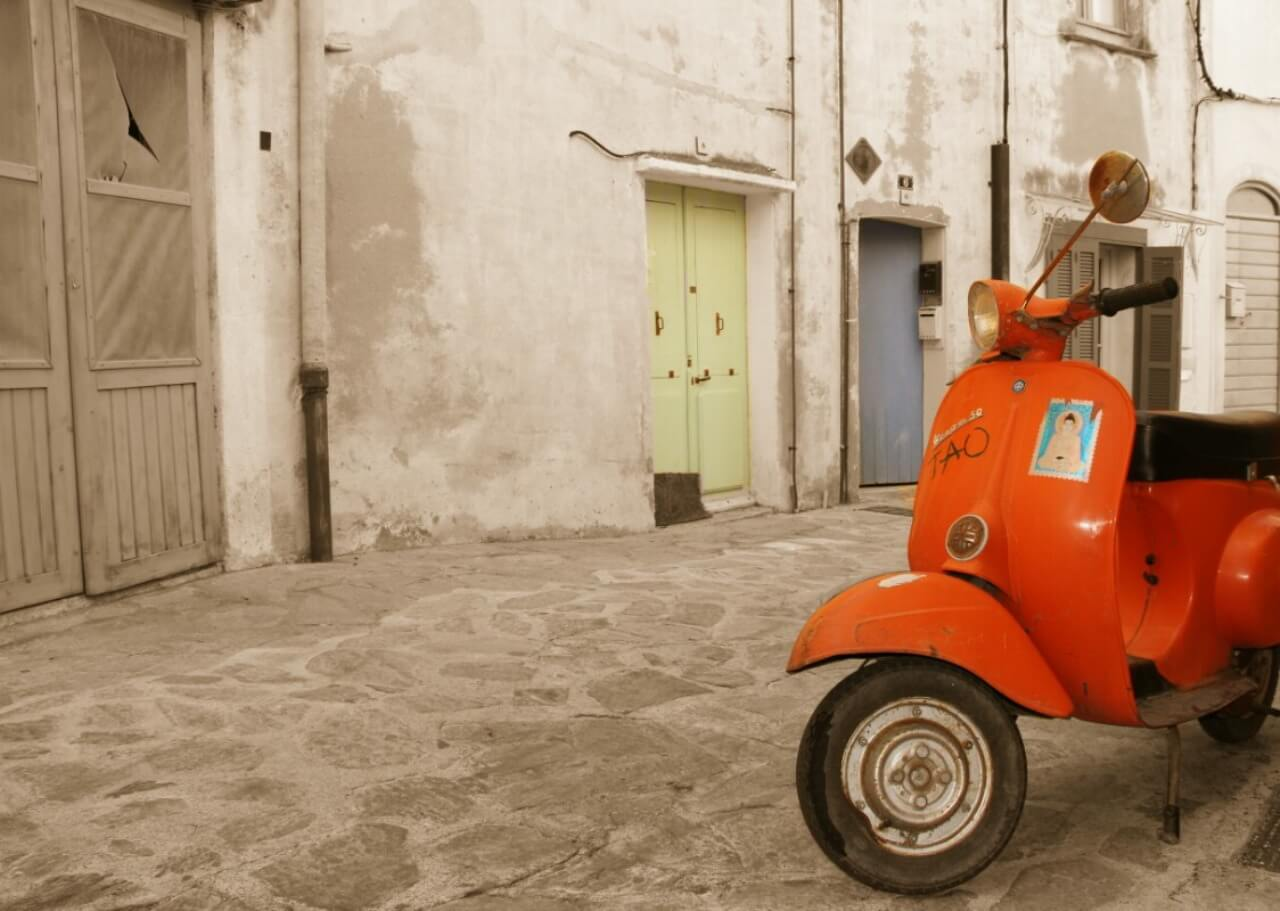
\includegraphics[width=\textwidth]{../Bilder/Korsika/25.jpg}
    \caption{Wunderbari Gässli}
    \label{img:Korsika2}
\end{figure}
\pagebreak

\subsection{08.09.2011 Donnerstag}

\begin{wrapfigure}{L}{0.45\textwidth} 
  \begin{centering}
    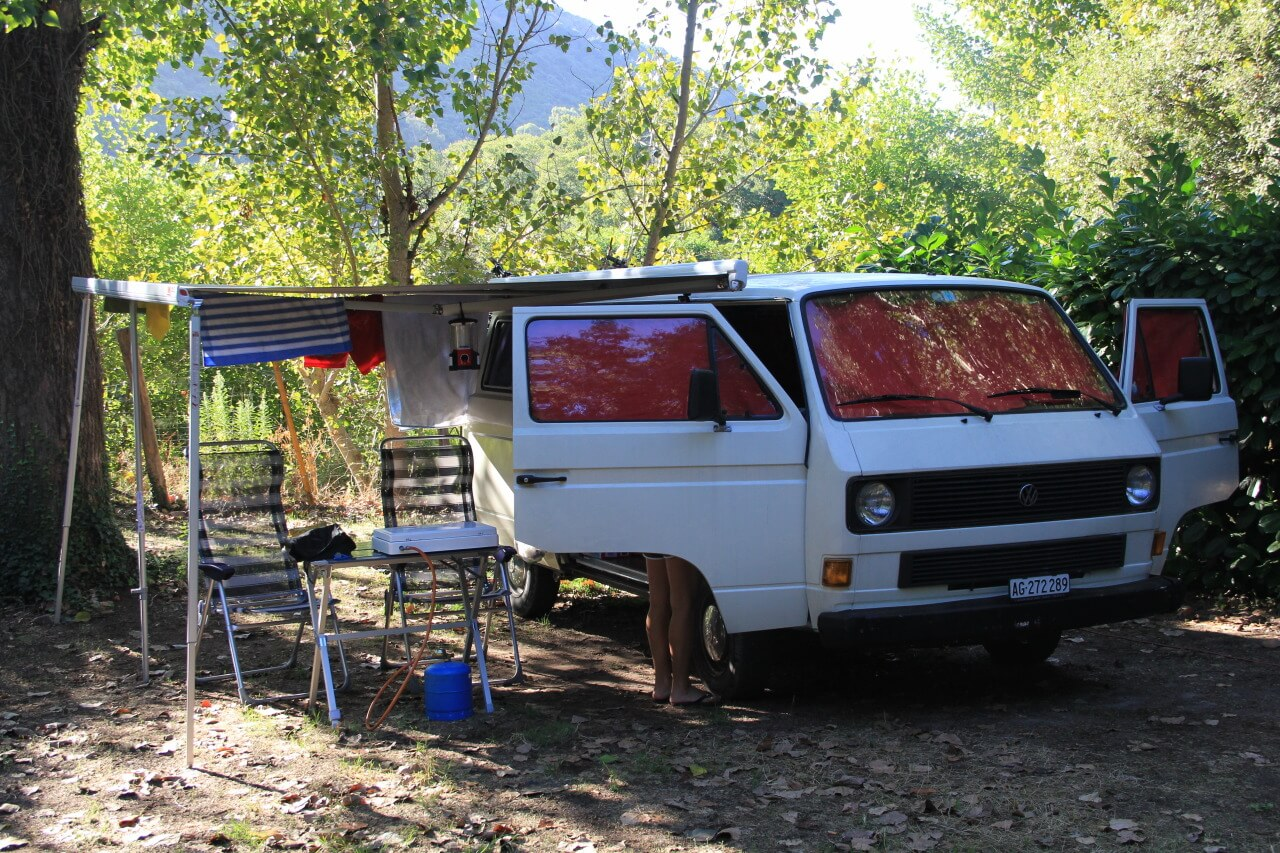
\includegraphics[width=0.4\textwidth, height=5cm, keepaspectratio]{../Bilder/Korsika/32.jpg}
    \caption{Jack in Action}
  \end{centering}
\end{wrapfigure} 

Scho am 8ti, so früüüe, semer ufgstande und hend eus los gmacht för en grossi Etappe.
Euses Ziel esch Porto gsi.
Ufem kurvige passähnliche Weg hämer es mega schöns Resti anere Bucht gseh und hend denkt, döt chömer schön zmörgele.
Es esch au woderschön gsi, nor de Weg zo dem Örtli esch zemliii steinig gsi.
Aber de Jack het da super öberstande.
Met wonderschöne Ussecht hemer en feine Kaffi gnosse.
Zrugg uf de Stross hemer witeri fantastischi Buchte erblickt und hend ufeme Ussechtsponk zmörgelet.
Es het weder es paar Föteli ge..damol sogar na vo Libelle und Schmetterling..ah nei vo Schmetterling ned, well de Herr Bopp vo dere wilde Kreatur devogsecklet esch rings um de Jack..
hihi die andere Touriste hend zemli komisch glueget.
Aber au ich be a dem Tag unter schlechtem Insekte-Zeiche gstande.
Min Wespistech, wo ich mer am Obe vorane leider zuezoge ha het afo bisse und na dezue send mindestens 2 witeri Ficher bem Fahre es Büsli gfloge und ich ha fasch es Herzchriesi becho.
Darum be ich die ganz Fahrt zemli verchrampft em Auto ghocked.
Leider het sich au euse Superdriver chli müesse verchrampfe, well ufem Weg nach Porto, zwoi riese Cars gmeint hend, sie müsset die winzig schmale und kurvige Küsteströssli ne! So hets natürli en riese Stau ge und alli hend vorwärts oder rückwärts en Nischeplatz müesse sueche.
Wo die superschlaue Cars verbi gsi send, hemer chöne witerfahre und send scho gli en Porto gsi.
De Golf vo Porto esch de schönst vo Korsika, aber leider daher au sehr touristisch.
dNatur esch wonderschön met de knallrote Granitfelse (Em Oste hets vor allem Schiefer(Meeressedimeten)) und em tüfblaue-türkise Meer.
Mer send dors Dörfli spaziert, am Genueseturm verbi, well mer döt hät müesse zahle und send an Kiesstrand ghöcklet.
Döt hemer leider ned chöne bade, well dWelle zu höch gsi send.
sGanze Dörfi esch eus vorcho wie em Europapark..ergendwie ned so atmosphärisch und eifach zemli könstlich.
Mer hend eus entschiede, gli weder ufzbreche und e chlini Wanderig em Calanche-Gebirge zmache.
Leider hets au döt zemli vell Lüt gha, aber die rot-orange Granitskulpture send schono idröcklich gsi.
Öpe e Stond em Ganze semer umegwaschlet und hend dFelsformatione, die steile Klippene und die wonderschöne Buchte bestunt.
Denn es witer gange richtig Sagone.
Eigentli hemer en Porto welle öbernachte, aber die velle Bluemchöl-Touriste und de Weg zrug hend eus dra ghinderet.
Mer send de witer dere schöne, chli enge Köstestross entlang be Piana und Cargese verbi, bes nach Sargone.
Döt hemer en grosse schöne Camping gfonde met Restaurant, Swimming Pool und Tennisplatz....nor send mer fasch allei gsi;) Zum Znacht hemer Omelette gmacht met Banane, Zucker und Zitrone.
Es esch supi gsi...hihi...nor het öper chli welle plöfe und het dOmelette ede Pfanne met Schwung müesse chere...leider het sich de Henkel glöst und die schön Omelette esch an Bode täscht...da het öper schön dumm glueget;) Devör esch öper andersch vom Campari chli gflasht gsi und hets chli lostig gha;) Fig und Fertig semer es Bettli plumpst.

\pagebreak

\subsection{09.09.2011 Freitag}

\begin{wrapfigure}{R}{0.45\textwidth} 
  \begin{centering}
    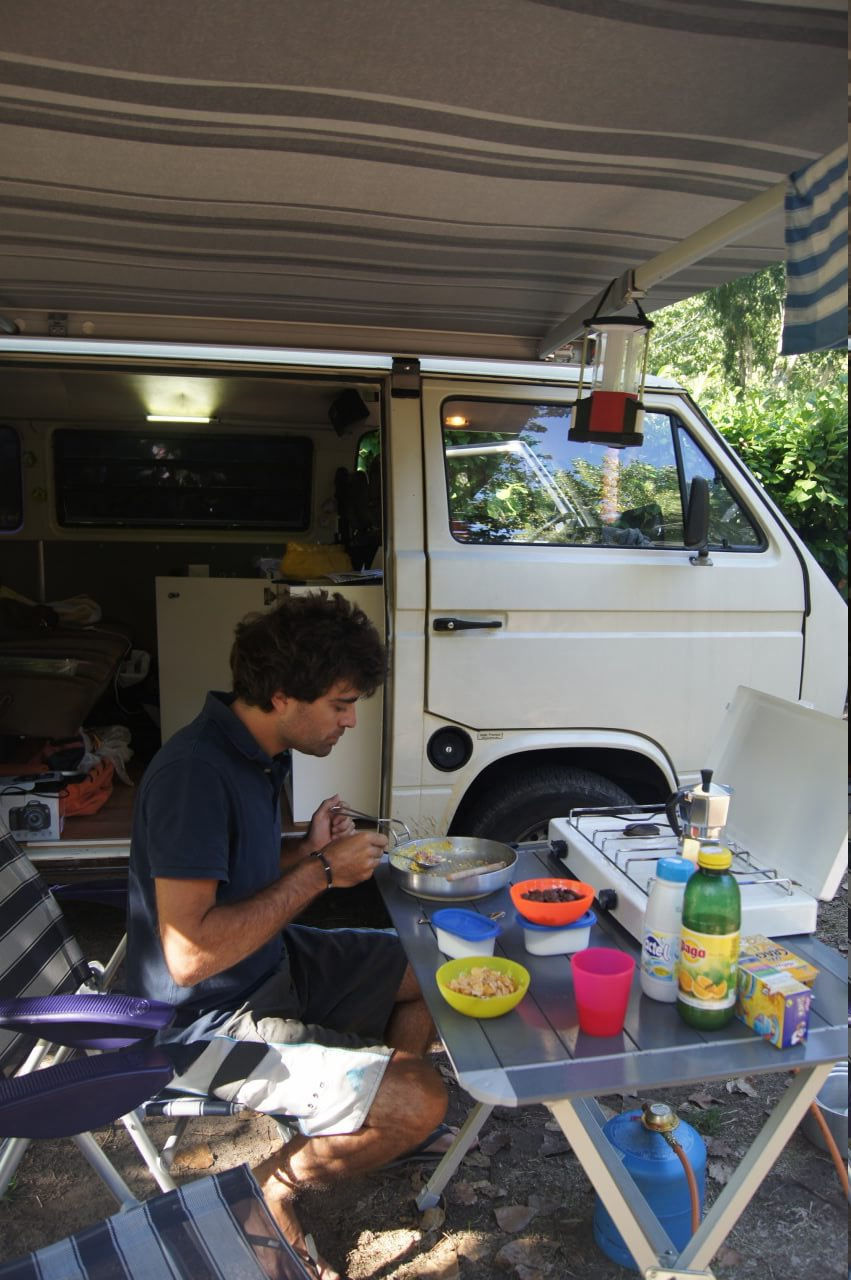
\includegraphics[width=0.4\textwidth, height=5cm, keepaspectratio]{../Bilder/Korsika/33.jpg}
    \caption{Zmorge}
  \end{centering}
\end{wrapfigure} 

Höt hemer feini Müesli und de Rescht vo eusere Omelette...Rüereier;) zum zMorge gha. 
Nachem zMörgele hemer scho gli mal welle anen Strand go eus erhole vo de gestrige Strapaze.
En Liamone hemer en wonderschöne Strand atroffe, wo Süess- und Salzwasser zämechond.
Schnell semer an Strand vöre und hend fasch nöme weg.
De Strand esch superschön gsi, sWasser glasklar und dWelle zemli gross.
De Pfödi het weder u Freud gha a dene Welle und esch rechtig go plantsche:) Mich hets au einisch schön am Strand nochezoge, was e sandigi Badhose met sich brocht het;) Speedminton hemer na versuecht zSpele, was be dem heftige Wind aber recht schwerig gsi esch.
Schliesslich hemer eus begnüegt met Fulenze, Lese und Sönnele...
die einte hends chli öbertrebe met de Sonne:-P Um di Drü semer witer nach Propriano.
Weder öber kurverichi Strössli semer de Köste entlang und de witer es Landesinner bes nach Ajaccio.
Vo döt het denn en grossi Strass nach Propriano gführt, was allerdings ned heisst, dass sie ke Kurve het und ned ufe gat.
Jetzt semer emene herzige Camping direkt am Meer grad vor Propriano am Strand vo Calanca.
Nacheme schöne Sonneuntergang am Strand hemer fein zNacht (Tortellini, Gurkesalat) kochet und hend damal en bessere Wy ganz wegputzt...uiuiui..das wär jetzt Stichwort gsi zum go pfuse;) Esch wedermal en superschöne Tag gsi..Hasta la vista:)

\subsection{10.09.2011 Samstag}
\begin{figure}[b]
   \centering
      %\subfloat[CAPTION]{BILDERCODE}\qquad
   \subfloat{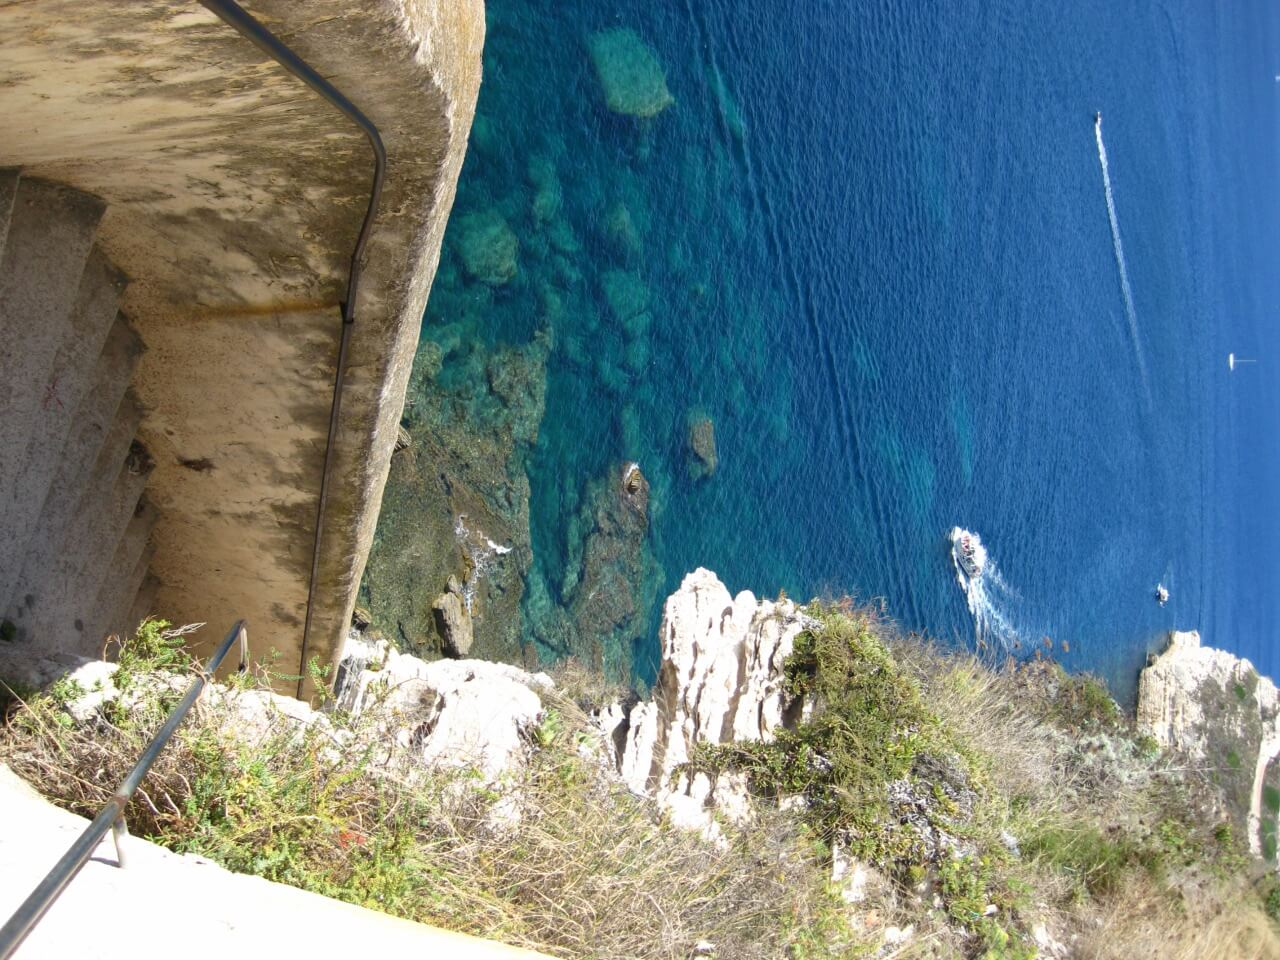
\includegraphics [width=0.3\textwidth]{../Bilder/Korsika/39.jpg}}\quad
   \subfloat{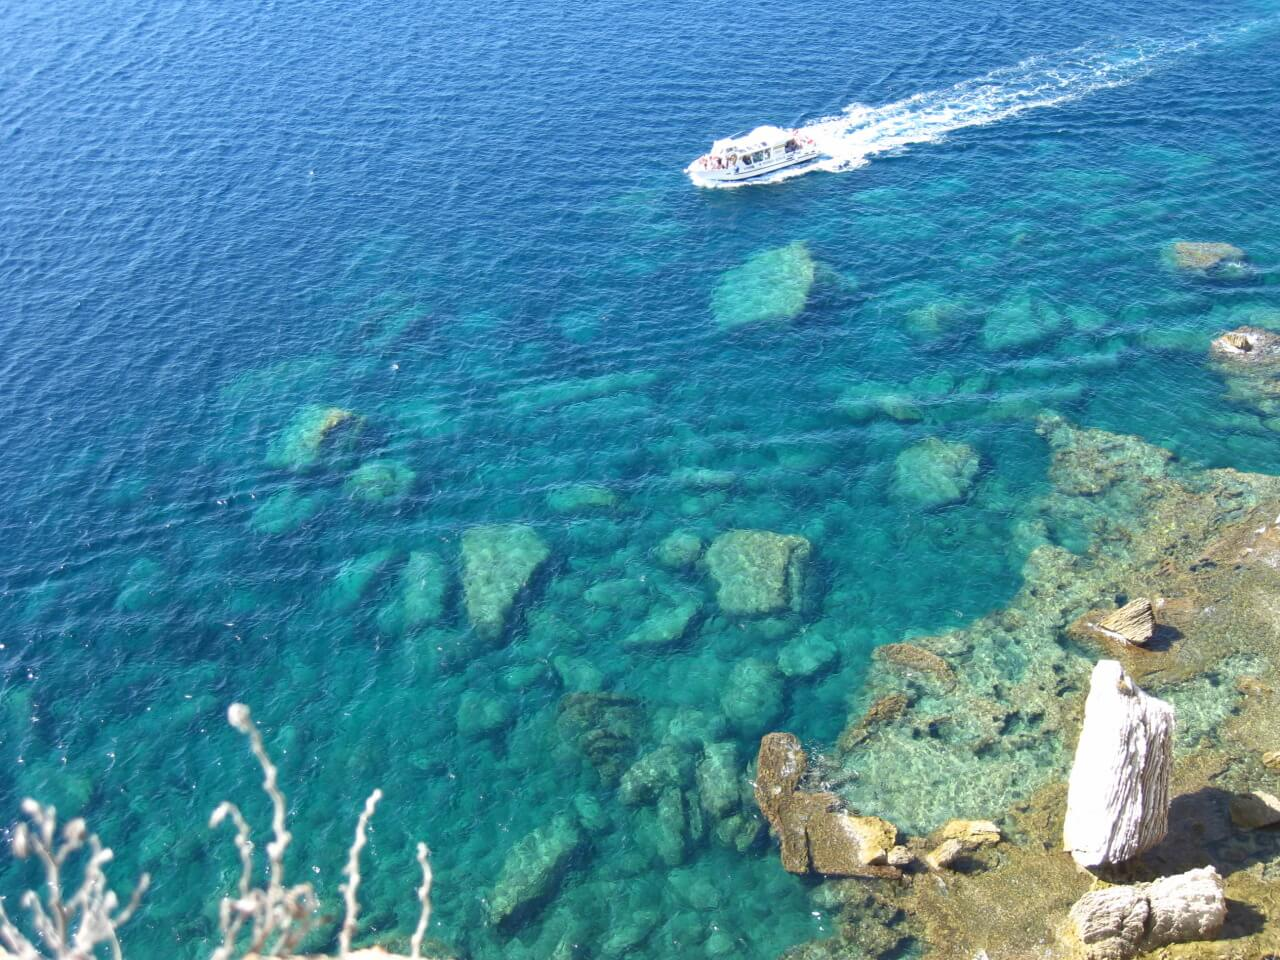
\includegraphics [width=0.3\textwidth]{../Bilder/Korsika/40.jpg}}\quad
   \subfloat{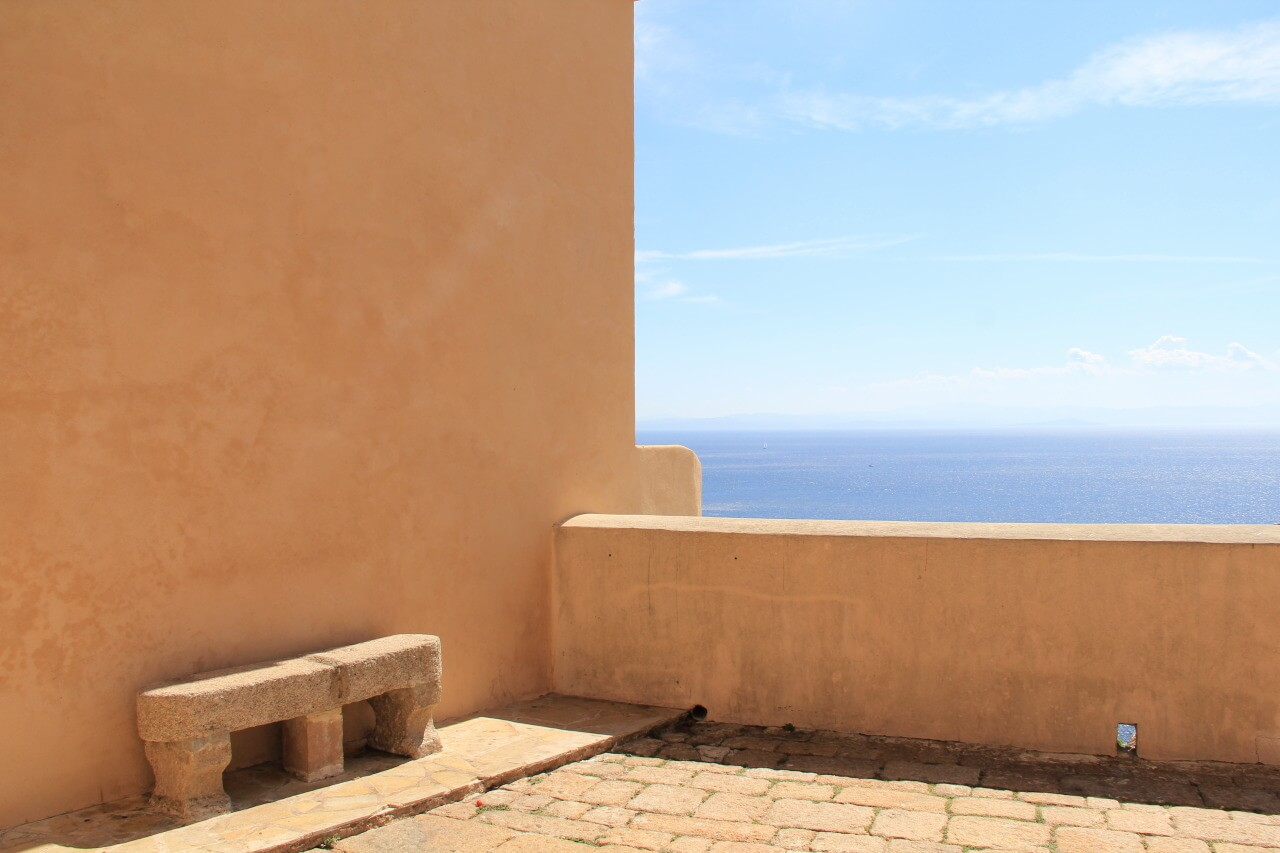
\includegraphics [width=0.3\textwidth]{../Bilder/Korsika/42.jpg}}\quad
   \caption[Idröck us Bonifacio]{Idröck us Bonifacio}
\end{figure}
Scho vor de 8tne semer höt ufgstande, wells ade Rezeption gester vo de sehr fröndliche Dame gheisse het, wer nachem 8ti zum Beck gat (ein Ma chond jede Morge met sine Brötli verbi), de chond norno Baguette öber. So simer fasch Ponkt 8ti zum Becker unter de Bäum und hend sogar na Croissant und Schoggi-Brötli ergatteret. Hmm...fein sends gsi:) Nachem zMorge semer an Strand ghöcklet und send e das glasklare Wasser go schwümme...esch wonderschön und erfrüschend gsi. Zrugg ufem Tüechli be ich scho gli ipfused und so eschs mer leider de ganz Tag gange...ich be entweder müed gsi, be en Trance gsi oder ha sosch chli umeträumt...en richtigi Schlafmütze be ich gsi. Aber mer hend trotzdem na es rechts Programm gmacht. Zersch semer es Zentrum vo Propriano go en Bankomat sueche. sStädtli esch recht touristisch, aber zemli herzig met de alte Granit-Hüser, de velle Lädeli und Gässli und em chline Hafe. De Bankomat esch zemli versteckt gsi, aber mer hend en schlussendlich doch na gfonde. Mer send de richtig Hafe glofe und hend em feine Duft vo de Bäckereie ned chöne widerstah. En Pizza, feini Zuckerbölleli und e Glace hets ge:) Nach dem Snack simer zrugg zum Jack und witer nach Sartene, skorsiste Städtli vo Korsika. Döt acho, hemer scho zemli schnell gmerkt, dass es wedermal sehr touristisch esch und mer fasch ke Parkplatz meh findet. Mer hend de doch na eine gfonde und send durs Dörfli gwagglet. Es het schöni, uralti und sehr engli Gässli, aber esch fast zu touristisch, chli wie em Europapark. Nachere Fotisession semer de au scho witer uf Bonifacio, de südlichst Ponkt vo Korsika! Zersch hemer na enere Bucht welle go schnorchle oder surfe, aber mer hend nor sone komischi versnobbti, chli langwilligi Bucht gfonde, wo mer ned wörkli het chöne go bädele. So semer witerzottlet und hend scho gli das wonderschöne uf Chridefelse baute Bonifacio erblickt. Da mer zersch uf euse Camping hend welle, send mer ade Stadt verbigfahre und send em Pfil Camping dIles gfolget....es esch ewigs gange bes mer denn endli bem Camping acho send. Em Reiseführer esch gstande mer cha met em Velo, evt. au zFuess ed Stadt laufe, aber da chömer also grad vergesse, es send öpe 8km uf Bonifacio, aber ufe und abe und vor allem ufe. Daher semer de grad do em Camping blebe und send met de Velo an relativ nöche Strand gradlet und send döt na es Stöndli umeglege. Eigenli hät die Bucht es Surferparadis sölle si, aber vo Wind und Welle hemer ned so vell gmerkt. Nachem fulenze und sönnele semer weder zu eusem Camping zrugdüset, go pöstele und hend zNacht kochet und zwar Ris met Chilli SENZA Carne. Da mer ned grad es mega Menü kochet hend, hemer denkt müemer devör umso meh bem trinke investiere;) de türst Wi bes jetzt (14 Euro) hemer kauft, was dVerkäuferi em Lade fasch gschockt het..sie het gmeint: "Cest le plus cher...tu as vu.??"ouioui:) Leider esch er gar ned so fein gsi und ich ha weg mim Chopfweh gar ke Lust meh gha uf Wi. Devör ha ich vo mim Schatz e heissi Schoggi becho:) hmm esch super gsi! De Steff het nachli glese und ich be wie en Stei es Bettli plumpst und sofort ipfuused.

\subsection{11.09.2011 Sonntag}
\begin{wrapfigure}{R}{0.45\textwidth} 
  \begin{centering}
    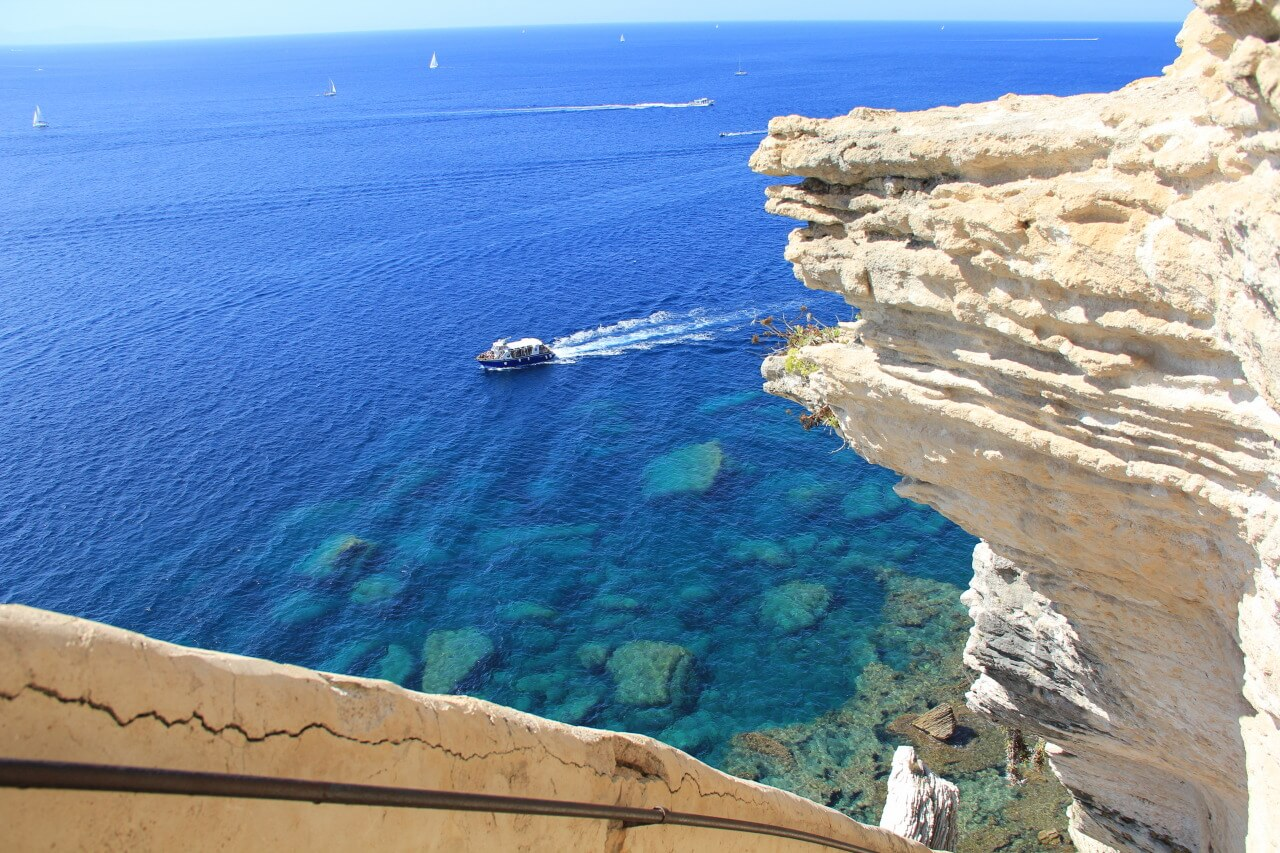
\includegraphics[width=0.4\textwidth, height=5cm, keepaspectratio]{../Bilder/Korsika/38.jpg}
    \caption{Bonifacio}
  \end{centering}
\end{wrapfigure} 
Höt hets feini Croissant und Schoggibrötli zum zMorge ge. Gmüetlich hemers gno und send de um di 11i uf Bonifacio..wow die Stadt esch echt de Hammer! Zersch semer am Hafe umegschlenderet, wo de Steff ganz vell riiiiesigi Jachte bestunt het und fasch chli ifersöchtig worde esch. Neb de Schiff hets ganz vell Restaurants, Kaffis und Bars gha. De simer ufegwanderet ed Oberstadt vo Bonifacio,wos eus gfalle het und mer paar Stöndli verbrocht hend. Bonifacio esch uf steile, zum Teil öberhängende Chridefelse baut und daher sehr imposant. De Ufstieg ed Altstadt esch dementsprechend au zemli astrengend gsi, abere het sich uf all Fäll glohnt. Die ganz Oberstadt esch nemli voll vo herzigi Gässli met vellne Restaurants, Souvenir-Läde und Kaffis. Zwösched inne hesch na en super Ussecht vode Chridefelse abe uf das traumhafte-glasklare Meer. Zum Zmettag hemer e chli en grossi Thunpizza und feini Crevette gha:) Denn semer na uf de Hügel visavis vode Altstadt gloffe und hend vo döt en geniali Ussecht uf dOberstadt unds Meer gha. Bem Abstieg ha ich fasch na es Herzchriesi becho, well churz vor mer en riiesige Schlange verbigschlänglet esch...uäää! De Steff het zersch nüt metbecho, well er sine Flugis nacheglueget het, ersch wo ich umegschroue und umegumpet be, het er sich gfragt, was e mich gfahre esch. Nach dem velle Umelaufe semer recht kaputti gsi und hend eus chli müesse ufeme Bänkli erhole. Da aber ersch 4i gsi esch und mer na hend welle zNachtesse en Bonifacio, hemer na paar Stöndli vor eus gha. Darum hemer denkt: Mached mer doch na e chlini Bootstour:) Am 5i semer de met eme Bötli usem Hafe gfahre und send grad e di erscht Grotte inegfahre..wow..türkis-glasklars Wasser, Tropfstei und Chridefelse..het superschö usgseh! De semer witer zode Lavazzi-Insle zo de Riche und Schöne und de weder zrug uf Bonifacio. Em schöne Obigsliecht het dAltstadt grandios usgseh und mer hend wedermal einigi Föteli gmacht. Mer het wörkli sGühl, die Hüser gheiet nächstens grad es Wasser. Die steil Aragon-Treppe hemer vo witem au bestunt. Die semer am Mittag abeglofe und send fasziniert gsi vo de schöne Felse und dem traumhafte Wasser. Nor vom Ufstieg semer de nöm so begeisteret gsi;) dBötlitour esch sehr erfröschend gsi. Trotzdem semer zrug em Hafe enes Kaffi go en Apéro neh...uiuiui...mer eschs nacher zemli guet gange;) Min Moon-Drink het echli vell Prosecco denne gha, so dass ich grad es Glas umgschmisse ha. Leider esch em Steff sin Rucksack dusched worde. De semer enes Resti gschwankt;) und hend sehr fein zNachtgesse. Damol hets Seetüfel met Pfeffersauce und St.Pierre met Nüssli und Ris und Gmües geh. Um di 10ni semer de zrug zo eusem Jack und uf de Campingplatz düset. Esch en superschöne Tag gsi:)

\subsection{12.09.2011 Montag}
\begin{figure}[b]
   \centering
      %\subfloat[CAPTION]{BILDERCODE}\qquad
   \subfloat{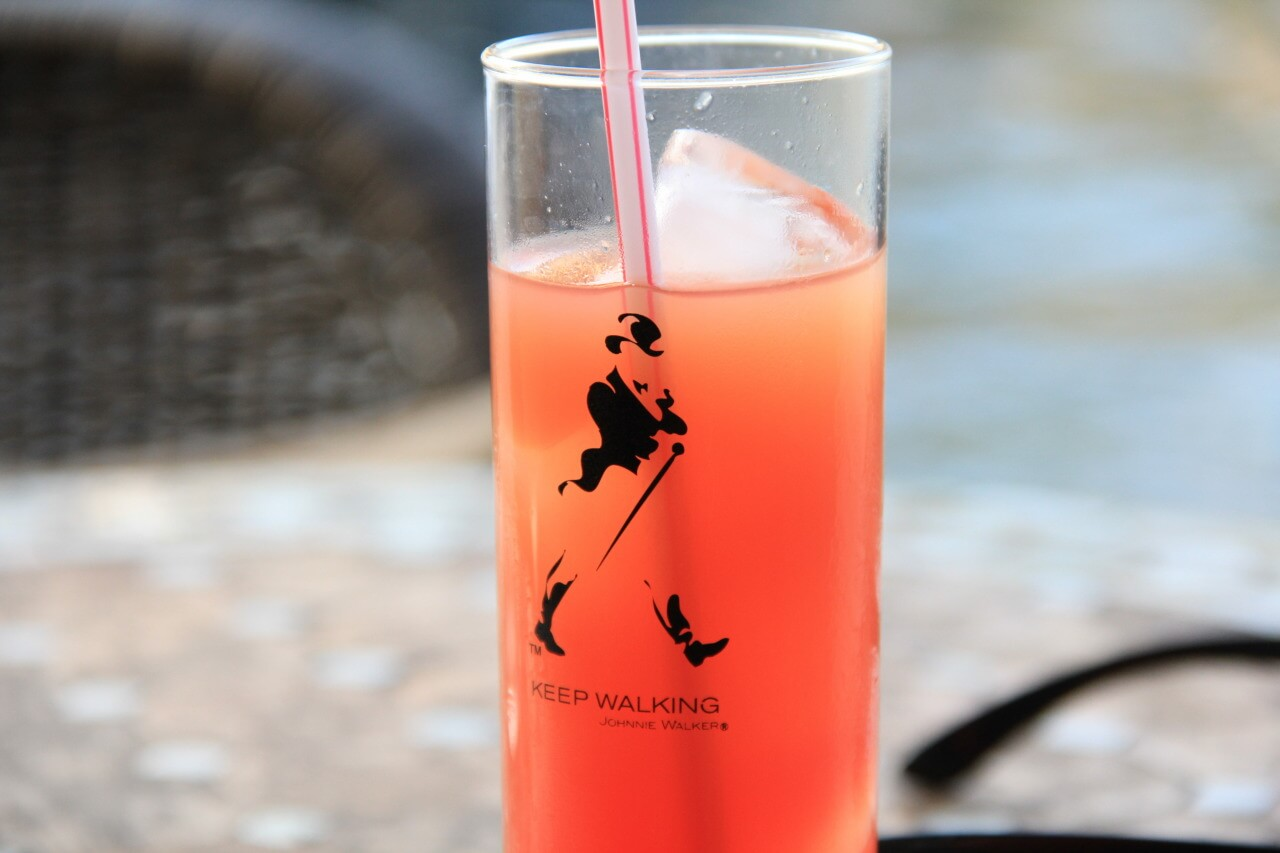
\includegraphics [width=0.3\textwidth]{../Bilder/Korsika/49.jpg}}\quad
   \subfloat{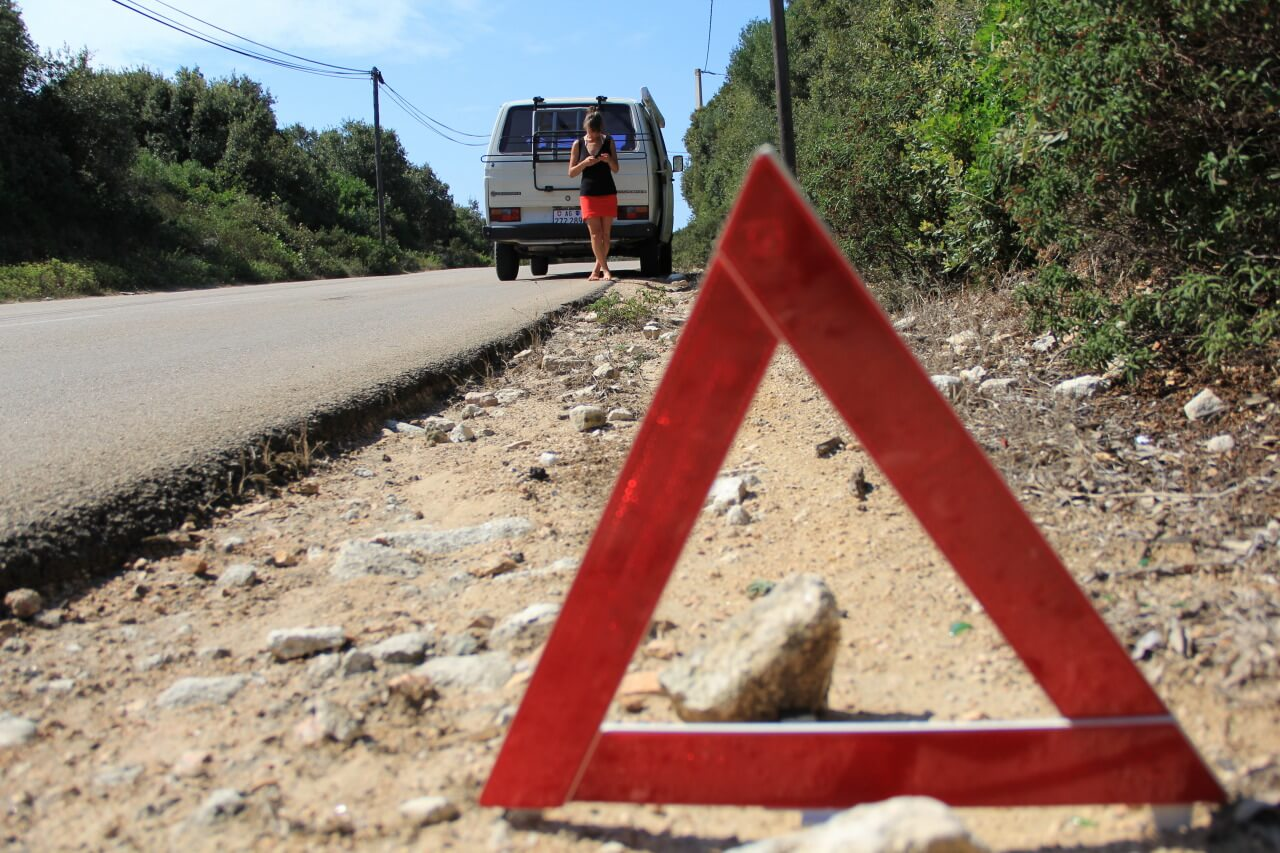
\includegraphics [width=0.3\textwidth]{../Bilder/Korsika/50.jpg}}\quad
   \subfloat{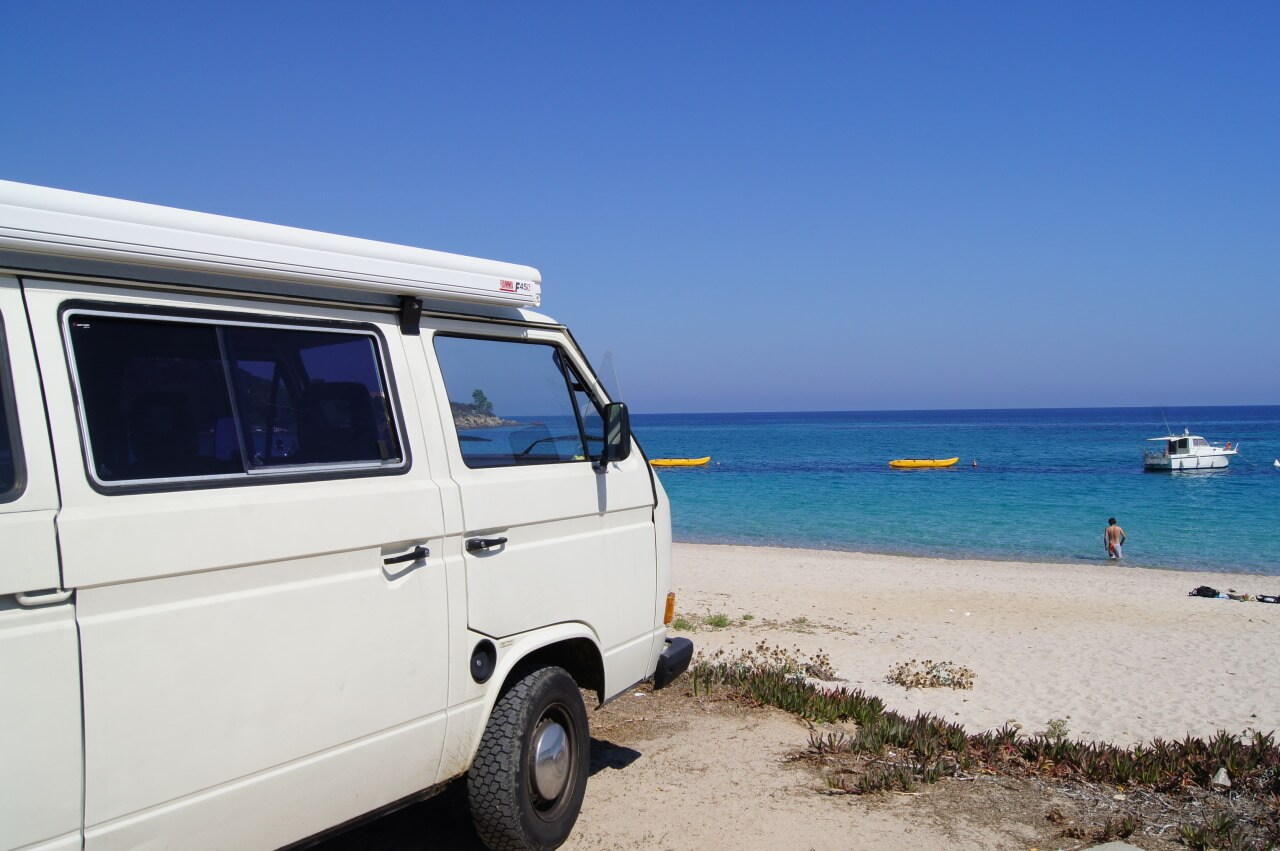
\includegraphics [width=0.3\textwidth]{../Bilder/Korsika/51.jpg}}\quad
   \caption[Pannentag]{Pannentag}
\end{figure}

Der Pechstag...fit und munter simer ufgstande,hend zmörgelet und hend eus uf de Weg nach Bonifacio gmacht.
Döt hemer ghofft en schrubeziehr zfinde, um dKeilrieme vom jack chöne zflicke,da de so komischi Grüsch vo sich get und internet, um mis Sprachmodul zBueche.
Beides hemer eigentli gschafft und trotzdem esch öpis ed Hose.
Ich ha am Hafe eme Internetkaffi chöne bueche und de Steff het zueffällig en chline Werkzüglade gfonde.
Glöcklich simer zrugg zu eusem Camping gfahre.
Ufem weg dethi hemer dKeilrieme na azoge und denkt;jetzt cha nüt meh schief ga;-) Leider hemer da falsch gedacht...
ufem Weg zo de superschöne Rondinarabucht,wo mer hend welle go bädele, het euse Jack schlapp gmacht:-\ dKeilrieme send grisse und de Motor het gsprudlet..ohoh..
Das het ned guet usgseh.
Nachdem de Steff es paar mal probiert het die Rieme weder anezmache unds ned klappt het, hemer eusi Hoffnige ufgeh und hend em TCS aglüte.
Die hend gmeint: e einere Stond werdet er abgschleppet.
So hemer e eusem Büsli gwartet und gwartet.
De esch endli sAbschleppauto cho...
de Fahrer het ke Muks gseit,het de Jack ufglade und eus gfrögt,öb mer wend metcho...
a klar hemer da welle,was hättet mer sosch sölle mache? Wo mer gfröget hend wos hi gat, het er gseit, nach porto veccio,döt säg di nöchst vw-garage.
Da simer grad chli verschrocke, da mer denkt hend mer gönd enen Werkstatt en Bonifacio.
Aber Porto Veccio esch nor e halb Stond entfernt gsi.
Be de VW Garage acho, esch de Jack abglade worde und de Schleppwaage esch schoweder abdüset.
Mer send de inne go frage, wie lang dReperatur werd ga, da hend si nome gmeint; höt werd er eh nüm aglueget, ersch morn morge und de meldet sie sich...
vorhe cha mer nüt säge.
Na super...so simer de Hügel ufe es Zentrum vo Porto Veccio zottlet und hend eus uf dSuechi vome Hotel gmacht.
Das esch gar ned so eifach gsi...
eis nachem andere hämer abklapperet,aber leider nüt gfonde, alles esch complet gsi! Scho fasch hemer dHoffnig ufgeh und eus met em Gedanke vertraut gmacht am Strand zschlofe, als em letzte Hotel womer gfröget hend, zwar au alles voll gsi esch, aber na es Abstellchämmerli frei gsi esch.
Natúrli hemer zuegseit und es esch gar ned so es chlises Zemmerli gsi.
Es het e Duschi, es WC(openair) und sogar en Fernseh gha.
Mer hend eus chic gmacht förs zNachtesse und send ed Altstadt vo Porto-Veccio.
Städtli esch wonderschön gsi met de velle chline,herzige und gmüetliche Restaurants,Kaffis und Lädeli, wo sich ede enge Gässli versteckt hend.
Znachtgesse hemer emene guete Resti ufere Terrasse, wo mer direkt uf de Hafe abe gseh het...wow...esch genial gsi!sEsse esch au himmlisch gsi! Mer hend grad es ganzes Menü gno: Rohschinke met Melone, Wildschweinlasagne, Penne met Lachs, Glace und Öpfelchueche.
De Vollmond esch de na ufgange und es esch en wonderschöne Obe gsi:-) Es het sich doch na zumene Glöckstag gwendet;-)

\subsection{13.09.2011 Dienstag}

\begin{wrapfigure}{R}{0.45\textwidth} 
  \begin{centering}
    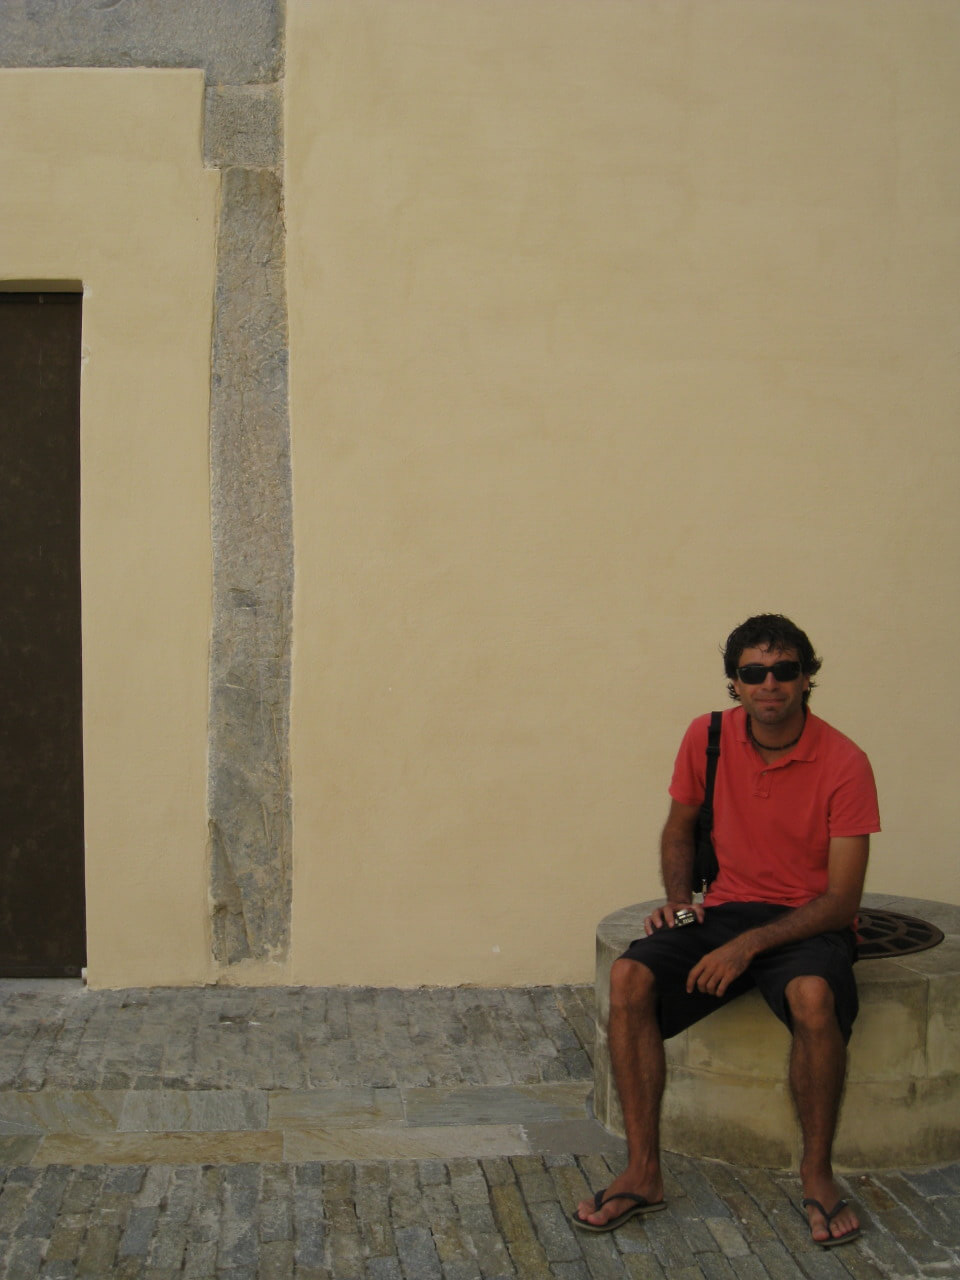
\includegraphics[width=0.4\textwidth, height=5cm, keepaspectratio]{../Bilder/Korsika/52.jpg}
    \caption{Ohni Bus unterwegs...}
  \end{centering}
\end{wrapfigure} 

Nachere vell zwarme Nacht und dementsprechend ned ganz so fit, simer uf de Garteterrasse vom Hotel fein go zmörgele.
Gstärkt simer ed VW Garage gloffe und hend ghofft, sie chönd eus scho meh Uskunft geh.
Aber wie erwartet esch na nix gange sie hend gseit, sie luegets am Namittag a...
uhh da ha ich schochli afo brodle und dampfe...
es het so tönt,wie sie en am donnstig mal alueget und de mal lueget was zmache esch und keilrieme wahrschinli na müend bstelle..grr..
mer hend de gseit, dass mer am Donnstig abreiset und so schnell wie möglich sött gmacht werde.
Serschte wo mer jetzt hend welle, esch es Mietauto gsi, well mer emmerna eusi Stüehl, Tisch und Velos em Camping be Bonifaciogha hend und mer müed gsi send vom velle umelaufe.
So hemer em TCS aglüte, welli eus versicheret hen, dass sie eus es Mietauto organisieretund wo eus grad be de Garage abholt.
WOW..das esch na Service hemer denkt und send erliechteret noimet abghöcklet und hend gwartet.
Nach öber e Stond hemer eus langsam gfröget, wo euses Auto esch, nach 2 Stond hemer namal aglüte.
De hets gheisse: ah ja ich ha ene grad welle alúte, sAuto staht parat bem Europcar! Jaja grad welle alüte, mer wartet 2 Stondund niemert informiert eus, echt en Frechheit! E dere Zyt hättet mer scho laang selber es Auto gmietet! Mer hend vermuetet, dass de Europcar bem Flughae esch und mer es Taxi múend sueche. Da mer aber kes Taxi gfonde hend, semer enes Resti und hend döt nach de Taxi-Telefonnummere gfröget.
Zum Glöck het sie eus de gseit, dass Europcar grad um de Ecke esch, zum Glöck! Aber da de ersch weder am 2 ufgmacht het, hemer nachli Zit múesse vertribe.
So simer nachli go shoppe:-) Mer send sogar erfolgrich gsi und es het neui Badhose, Hemdli und Flipflops geh.
Sauto hemer am 2 chöne abhole und so simer de au endli eusi verlorene Campingsache go hole.
Da mer eigentli scho laang hend welle go bädele, simer de na gschnell an Strand ghöcklet.
Denn het de Steff e suuuper Nachricht becho: Euse Jack esch gflickt und abholbereit,jupiii! Schnell simer zode Garage düset, hend de Jack gholt, sMietauto weder zruggeh und de schöni Camping Rondinara gfahre.
Döt hemer fein zNachtgesse(Tortellini) und send de gli go pfuse, da mer zemli müed gsi send.
Aber au sehr glöcklich, well mer euse Jack weder gha hend:-)

\subsection{14.09.2011 Mittwoch}
Strandtag, jupiii :) Höt semer de gaaaaaaaanz Tag am wonderschöne Rondinarastrand glege, hend gsönnelet und bädelet.
sMeer esch glasklar und so schön türkis gsi, wie uf de Maledive.
Zum Bade esch es eifach traumhaft gsi.
Nebem ful umelege, hemer nachli Speedmington gspelt, was aber dank em Wind gar ned so eifach gsi esch.
Denn semer na go schnorchle.
De Steff esch extra am Mittag be grösster Hitz de steil Weg zum Camping ufegloffe und het eusi Schnorchelsache...
leider hets sich ned glohnt, well mer ussert paar chline Feschli und es paar Felse ned vell gseh het.
Devör hets sich glohnt, dass mer es Bodyboard kauft und mitgschleikt hend.
Wells ade Ostküste sooo hochi Welle gha het, hemer eus eher gfühlt wie gstrandeti Wale als wie Surfer;-)
Zmettaggesse hemer em schöne Strandrestaurant.
Um di 6i semer zrug zo eusem Camping und hend euses zNacht vorbereitet, Ratatouille met Ris und feinem Rosé.
Nachem Esse hemer na öber Gott und die Welt plauderet und send de ab es Bettli..
met emene chli warme, sonneuftankte Chopf.
Ou öpis hani na vergesse...
mer hättet eigentli super gschlafe, wenn euse liebi Nachbar, wo zersch e Liechtshow abzoge het, ned so lut gschnarchlet hätt, dass de ganz Camping bebt hätt und am Morge rings um en ume alli gflüchtet send.

\subsection{15.09.2011 Donnerstag}
Höt heisst ab nach Bastia! Früe semer ufgstande und hend eus uf de Weg gmacht in Norde vo Korsika.
Zersch esch de Steff die voll krassi und kurverichigi Stross vom Camping zruggfahre und witer bis zume superschöne Sandstrand nördlich vo Porto Vecchio.
Döt semer zum letschte Mal namal e das wonderschöne Meer gumpet und hends eifach gnosse.
Denn han ich denkt, jetzt cha ich witerfahre, send ja schöni, gradi und breiti Strasse...
esch au alles guet gange, bes mich es fetts Hummeli es Födli gstoche het! Auuuua! Ich be ufgspronge, has Stürrad losglo, has Hummeli wegworfe und da hets mi grad namal en Finger gstoche! De Steff hets Stürrad müesse überneh, denn ha ich mich weder chli beruhigt und be uf dSite gfahre, usgstege und umegsprunge...haha..
de Steff het weder müesse witerfahre und ich hami nebeddra versuechts erhole..
was gar ned so eifach gsi esch, wenn mer ned ufs Födli cha hocke:-P
En Bastia acho, semer namal chli an Strand ghöcklet und send de es Zentrum an Hafe go zNachtesse.
Nachem Esse hemer na en Camping müesse sueche und hend eus för de stadtnöchsti Platz entschede, wo ned wörkli schön gsi esch, aber devör direkt am Meer.

\begin{figure}[H]
    \centering
    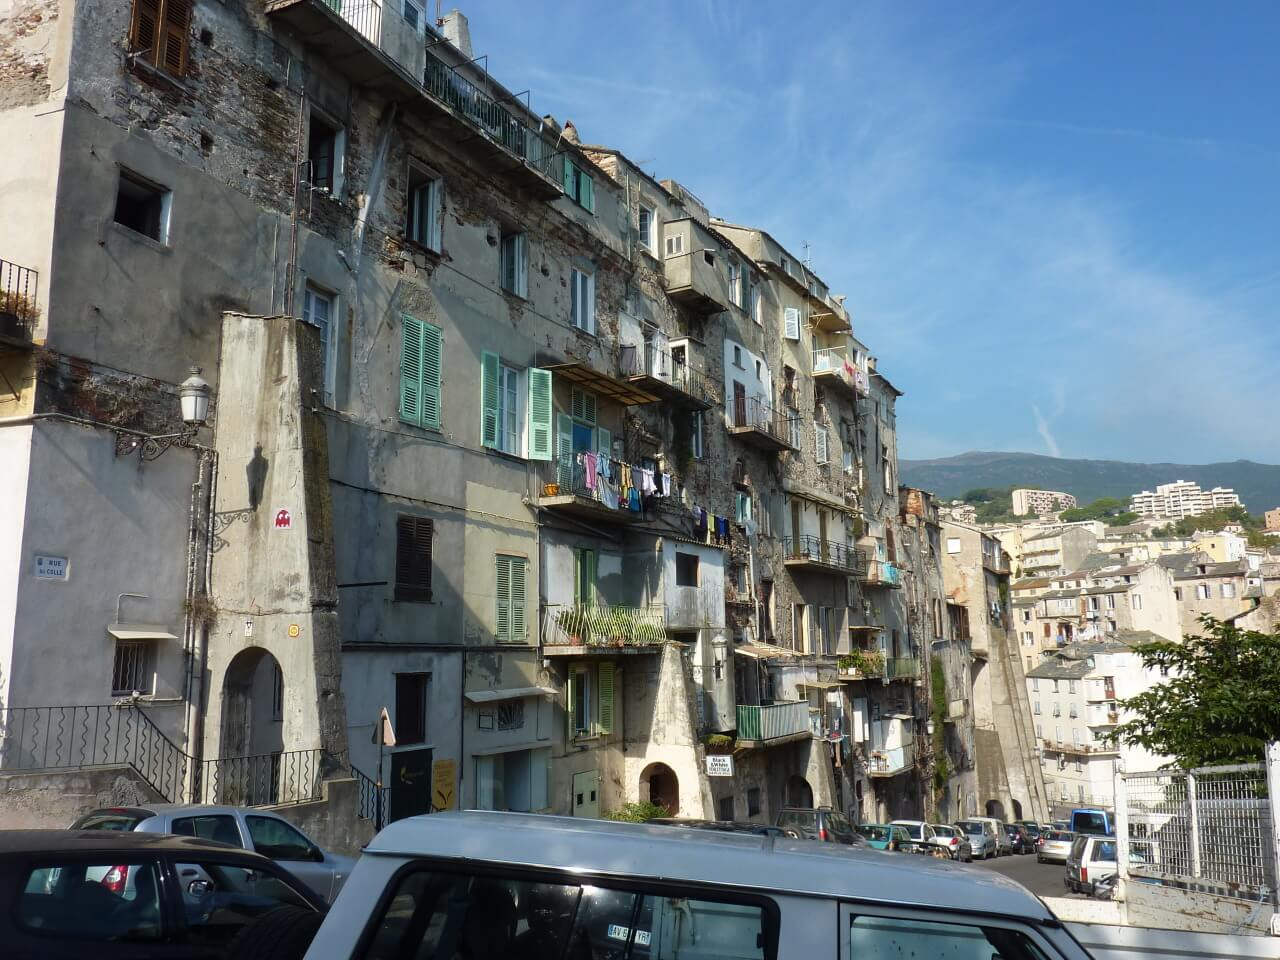
\includegraphics[width=\textwidth]{../Bilder/Korsika/53.jpg}
    \caption{Bastia}
    \label{img:Korsika3}
\end{figure}

\subsection{16.09.2011 Freitag}
Höt morge hemer die schöne sanitäre Anlage vo eusem super Campingplatz kenneglernt...
wuäää und de hends na neb eus sAbwasser abgloh.
Mer send de schnell uf Bastia innegfahre und hend ede schöne Altstadt zmörgelet met wonderschöne Ussecht uf de Hafe.
Mer send nachli ede Stadt umegschlenderet und hend de dFähri ufgsuecht.
Die esch lang ned ume gsi, het sich de aber doch na blicke lo und de esch alles schnell gange.
Schlossendlich semer fascht rechtzitig abgfahre.
Mer hend euse Jack parkiert, send ufs Deck gstörmt und hend na en Platz ergatteret zum sönnele:) Die nächste 5 Stond hemer met lese, sönnele, Bricht schribe und esse verbracht;) En Genua acho, semer grad witergfahre durs Aostatal, wo mer fasch uf jedem Högel schönbelüchteti Ruine gseh hend und dur de Gross Sankt Bernard, was 35 Franke kostet het.
Uf Sion het sichs de doch na lang zoge.
Ersch am halbi 2 semer en Sion acho und hend nebere Fabrik es Öbernachtigsplätzli gfonde.
Müed vode lange Reis, aber gspannt uf dFlugshow morn, semer grad es Bett gheit und ipfused.

\begin{figure}[H]
    \centering
    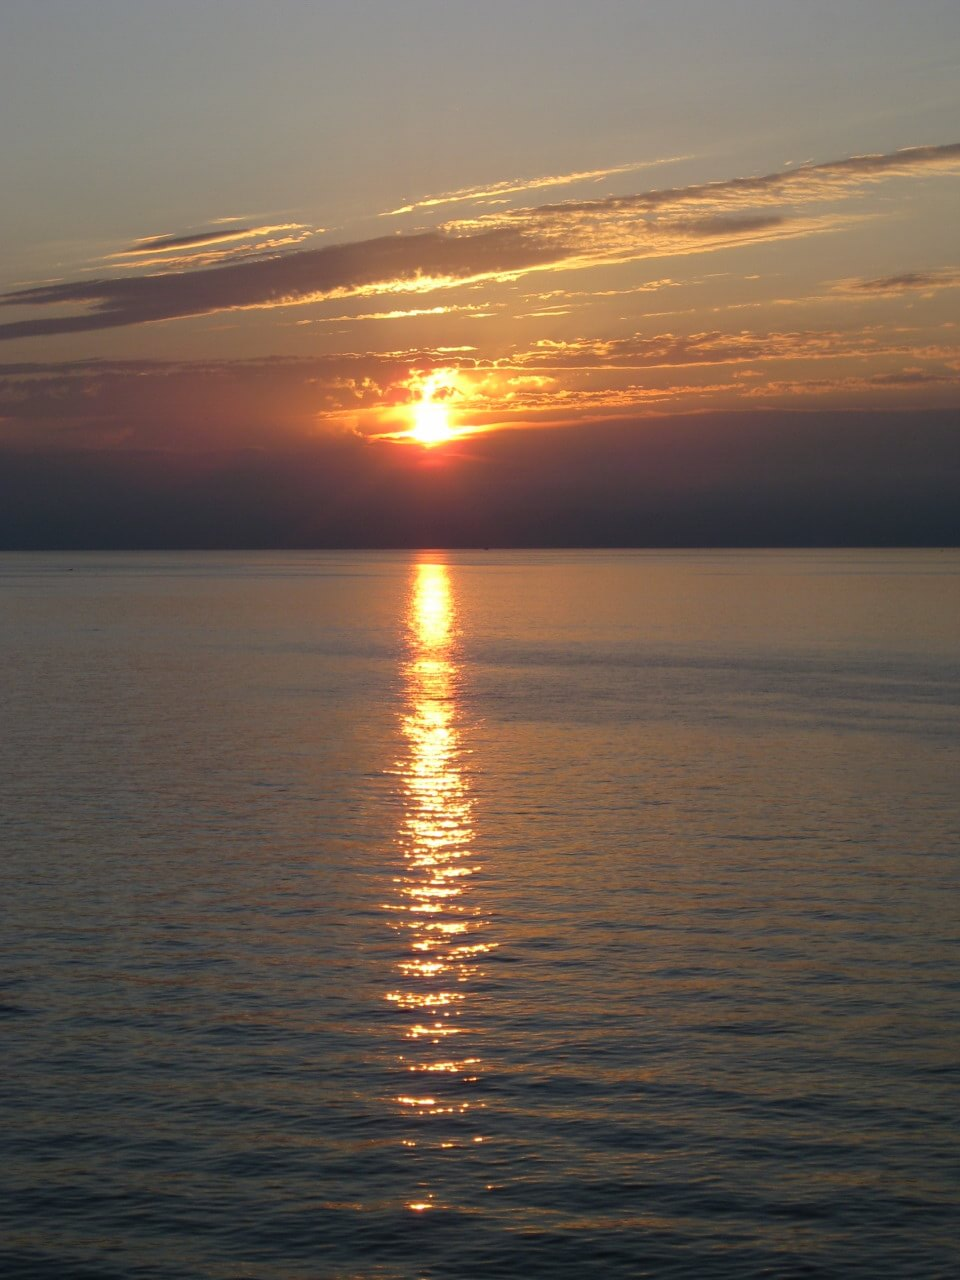
\includegraphics[width=\textwidth]{../Bilder/Korsika/54.jpg}
    \caption{Herrlichi Ferien gsi}
    \label{img:Korsika4}
\end{figure}
